\documentclass{beamer}
%
% Choose how your presentation looks.
%
% For more themes, color themes and font themes, see:
% http://deic.uab.es/~iblanes/beamer_gallery/index_by_theme.html
%
\mode<presentation>
{
  \usetheme{Boadilla}      % or try Darmstadt, Madrid, Warsaw, ...
  \usecolortheme{default} % or try albatross, beaver, crane, ...
  \usefonttheme{default}  % or try serif, structurebold, ...
  \setbeamertemplate{navigation symbols}{}
  \setbeamertemplate{caption}[numbered]
} 

\usepackage[english]{babel}
\usepackage[utf8x]{inputenc}
\usepackage{booktabs}
\usepackage{multirow}
\usepackage[scale=2]{ccicons}

\AtBeginSection[]
{
  \begin{frame}<beamer>
    \frametitle{Plan}
    \tableofcontents[currentsection]
  \end{frame}
}
%\AtBeginSubsection[]
%{
%  \begin{frame}<beamer>
%    \frametitle{Plan}
%    \tableofcontents[currentsection, currentsubsection]
%  \end{frame}
%}

\title[Patent Mining]{Classifying Patent Based on their Semantic Content \\ An empirical exploration into patent text mining}
\author[Bergeaud, Potiron, Raimbault]{Antonin Bergeaud \and Yoann Potiron \and Juste Raimbault}
\institute[]{Banque de France, Keio University and ISC-PIF}
\date[14/12/2018]{Computational and Financial Econometrics\\
Session Text Mining\\
14 December 2018}

\begin{document}

\begin{frame}
  \titlepage
\end{frame}

\section{Introduction}

%\begin{frame}{Motivation}
%    %Patenting is increasing, big data blablabla
%    
%    \textit{Patenting as a footprint of technology and its coevolution with science and culture~\cite{bais2010praise}}
%
%\bigskip
%\centering
%
%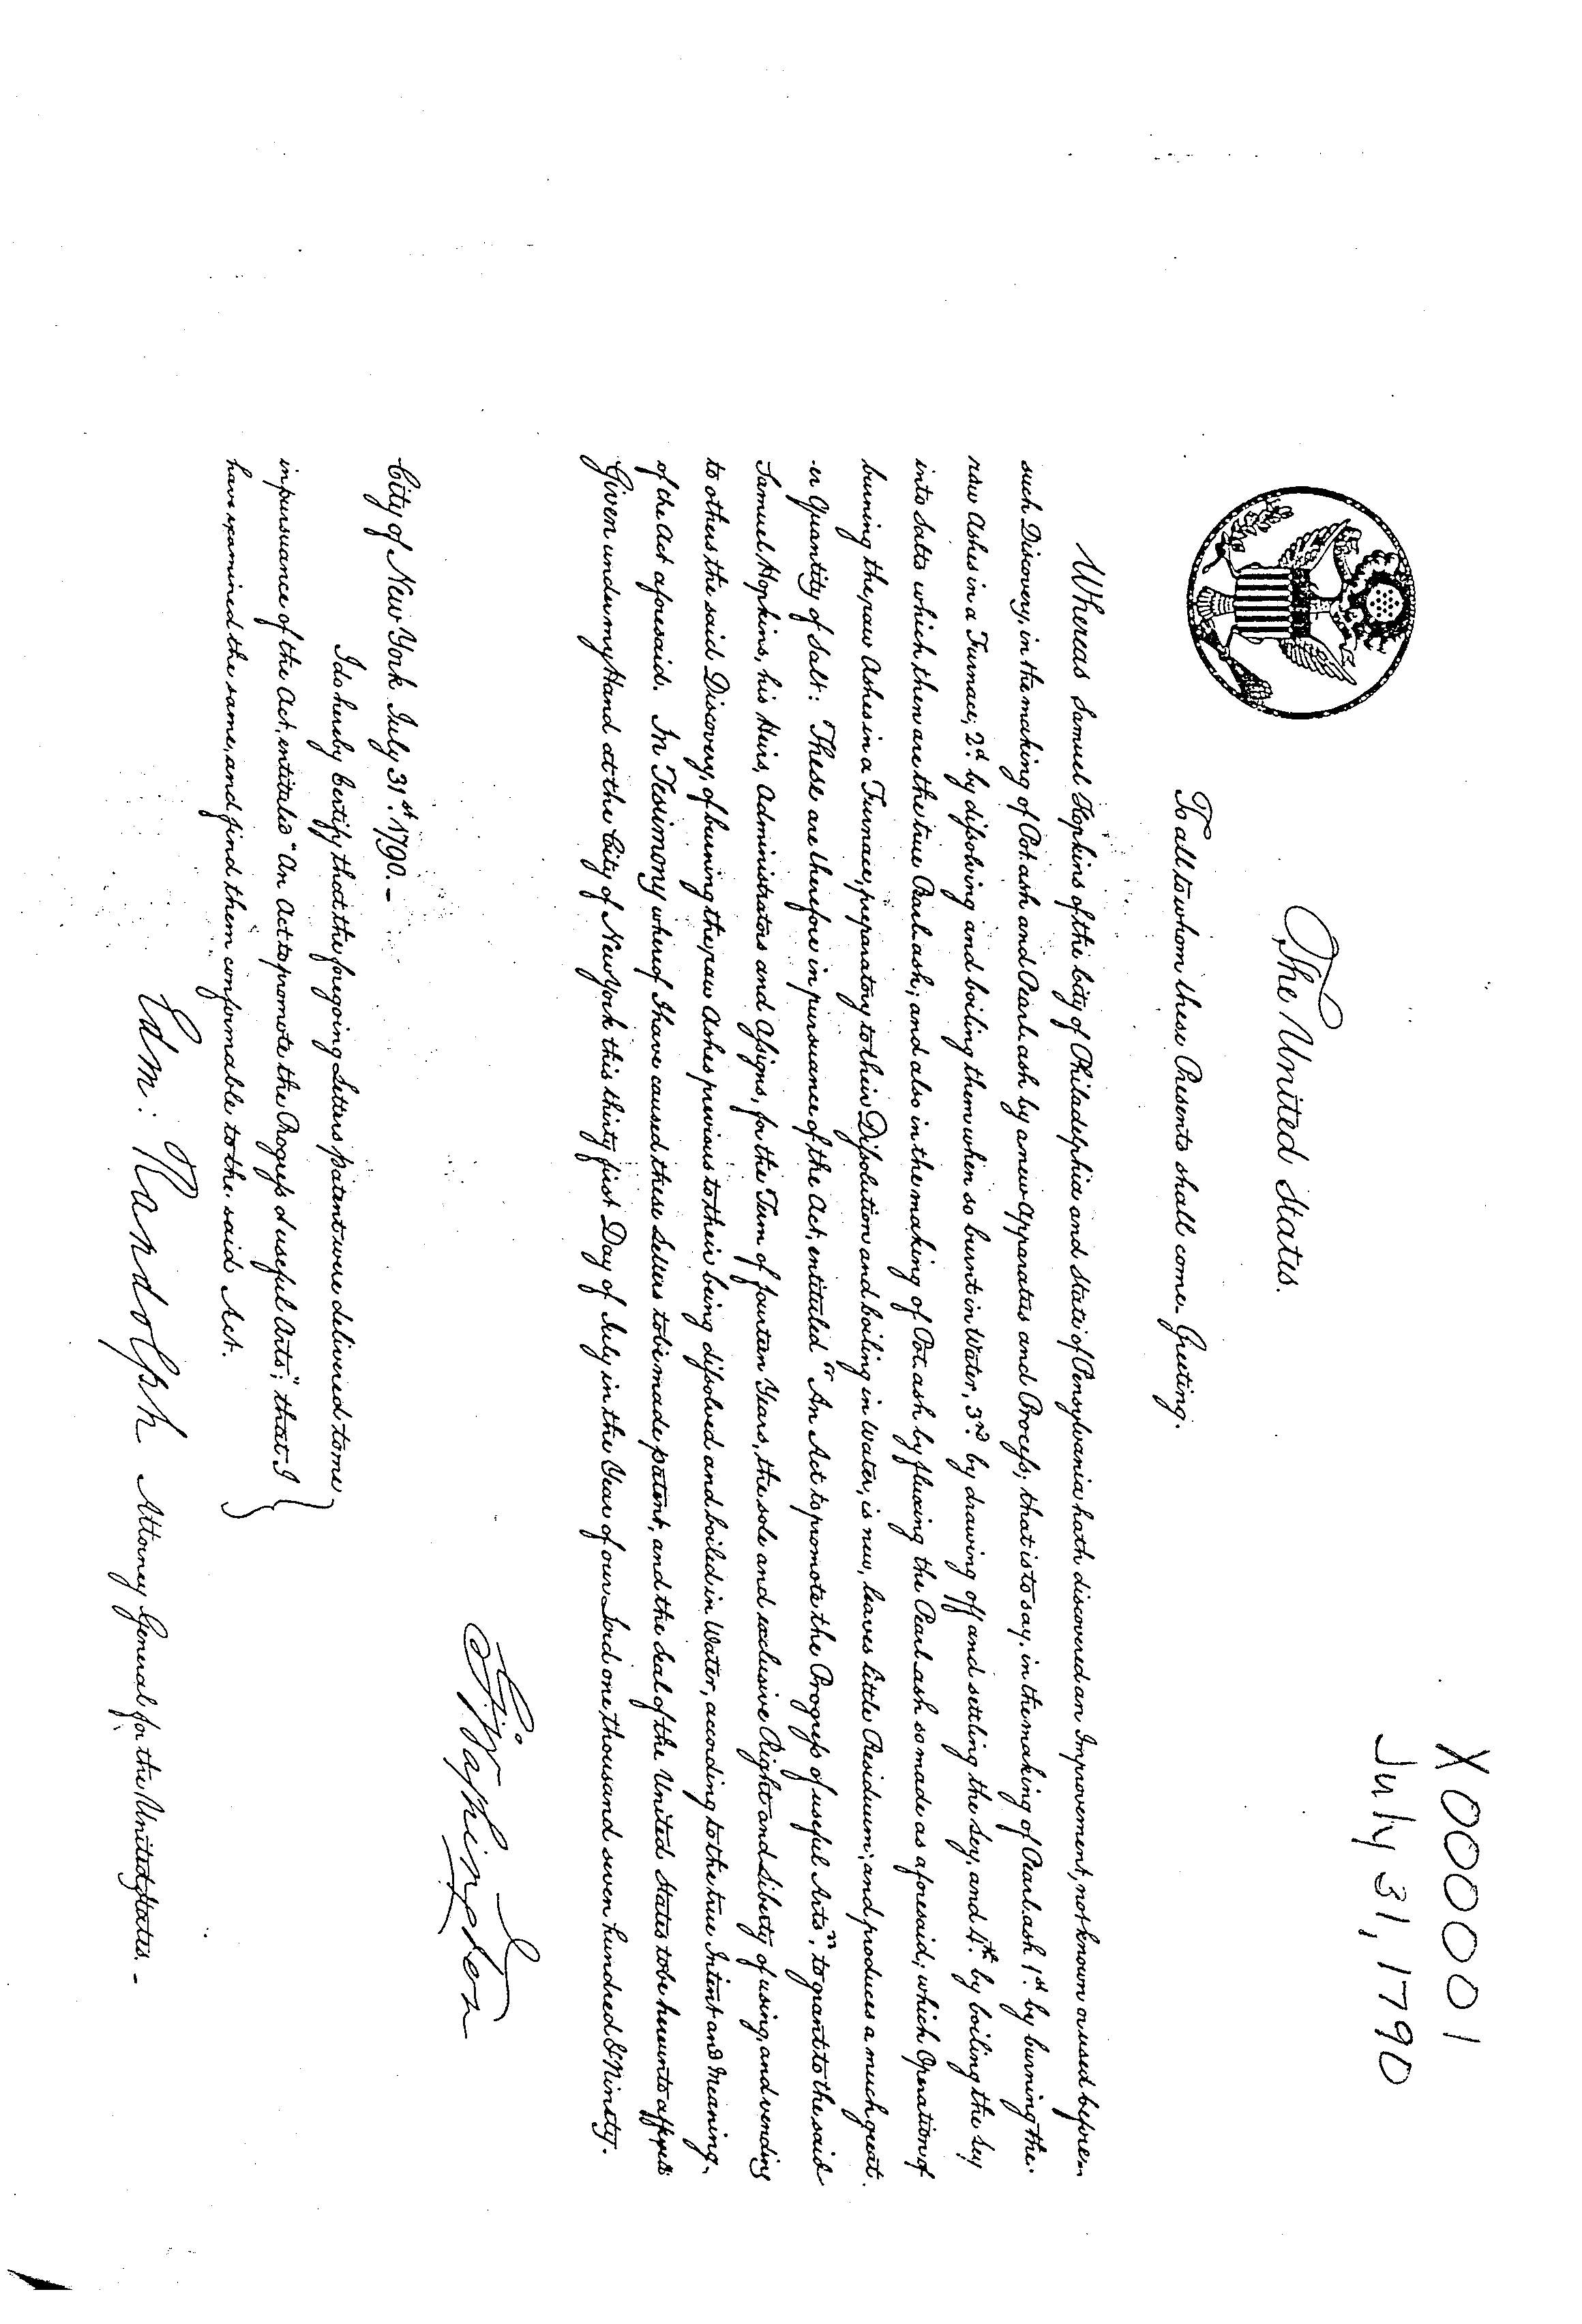
\includegraphics[width=0.35\textwidth,angle=90]{figures/USX1}
%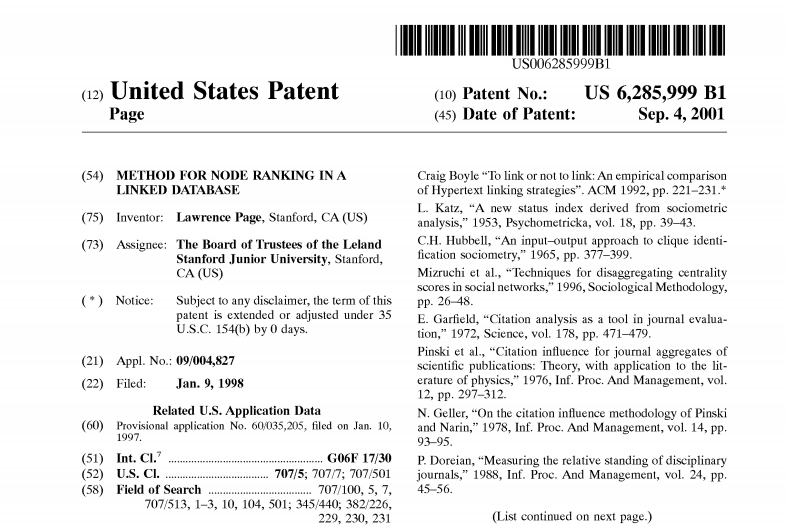
\includegraphics[width=0.45\textwidth]{figures/pageRank}
%    
%\end{frame}
\begin{frame}{Motivation}
    \begin{figure}
        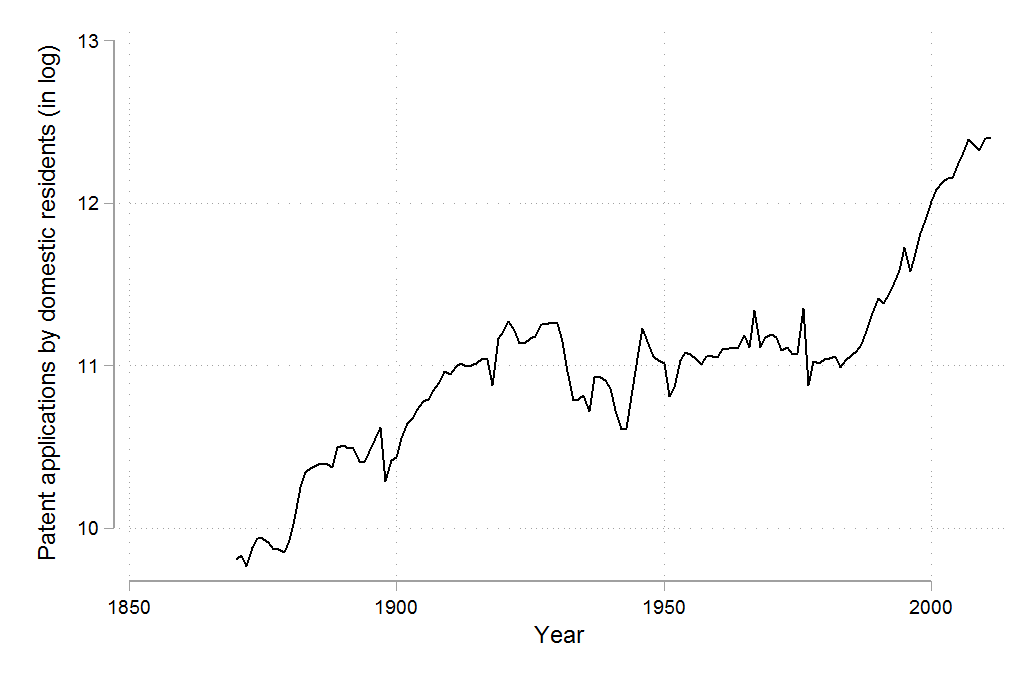
\includegraphics[width=0.8\linewidth]{figures/patent_usa.png}
        \caption{Log number of patent applications per capita at the USPTO. Source : USPTO}
    \end{figure}
\end{frame}
\begin{frame}{Motivation}
What are patents?
\begin{itemize}
    \item Property rights to an invention (novelty, non-obviousness and industrial applicability). Set the state of the art of a technology.
    \item Classification system in technology fields (or classes).
    \item Concept of ``Person having ordinary skill in the art'': an invention must be sufficiently disclosed in the description of the patent.
    \item Different realities between countries/IP offices (USPTO, EPO, JPO, CNIPA...).
\end{itemize}

In practice, patent data are available in the form of a relational database.
\end{frame}
\begin{frame}{Motivation}
    \begin{figure}
        \centering
        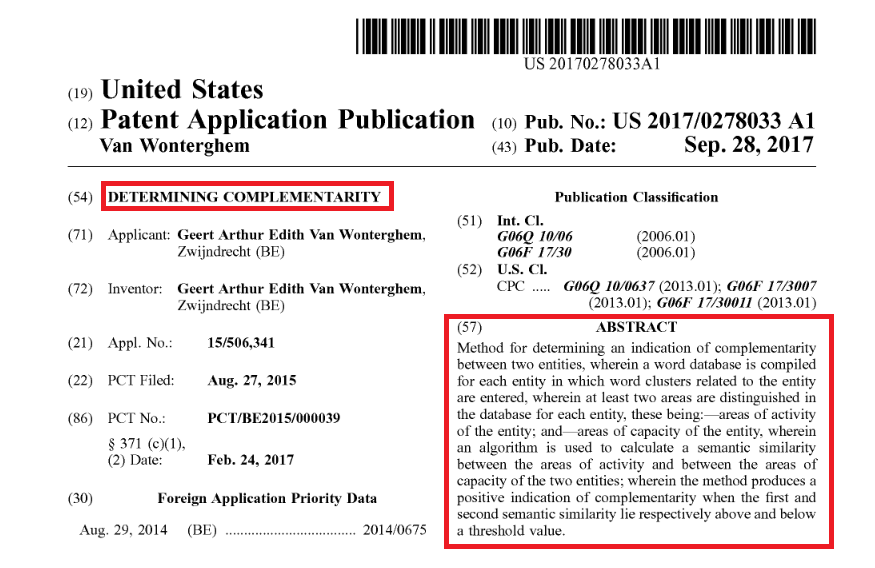
\includegraphics[width=0.8\linewidth]{figures/patent_abstract_ex.png}
        \caption{Example of patent front page. Source : USPTO}
    \end{figure}
\end{frame}
\begin{frame}{Why study patents ?}

$\rightarrow$ Although imperfect, patents are the most commonly used measure of innovation in economics. \\ % return to innovation, matching with firms, citation analysis...
$\rightarrow$ Applied Epistemology : particular case of the ecology and evolution of knowledge; diffusion of knowledge.

\bigskip

\textbf{Patents and text-mining: }

    \begin{itemize}
        \item Main usage: matching between patents and firms/inventors
        \item Used in the search of prior-art/litigation
        \item Technology mapping
    \end{itemize}
\end{frame}

%\begin{frame}{Why study patents ?}
%\textbf{\textcolor{red}{virer ?}}
%\justify
%
%$\rightarrow$ Although imperfect, patents are the most commonly used measure of innovation in economics. \\ % return to innovation, matching with firms, citation analysis...
%$\rightarrow$ Applied Epistemology : particular case of the ecology and evolution of knowledge; diffusion of knowledge.
%\bigskip

%\textbf{Examples :}

%\begin{itemize}
%\item \cite{griliches1998patent}: patent as an economic indicator
%\item \cite{Youn:2015fk} interaction between technological fields ; combinatorial nature of inventions
%\item \cite{2016arXiv160207928B} citation network analysis to detect emerging research front
%\item \cite{gerken2012new} \cite{tseng2007text} semantic analysis (remains limited to specific fields and time windows)
%\end{itemize} 
%\end{frame}


\begin{frame}{A large scale semantic insight into USPTO database}
    
    % integrer le ``what we do'' ici ?   
    
    \textbf{Proposed approach}
    
    \medskip
    
    \textit{Complement existing patent office classifications using patent semantic content} \\
    \textbf{Why?}: more endogenous, flexible and informative (?). And comparison with \emph{technological} classification to detect outliers.
    
    \bigskip
    
    \textbf{Takeaway results}
    
    \medskip
    
    $\rightarrow$ \textit{An endogenous semantic classification is constructed for the full USPTO abstracts and titles, 1976-2012}
    
    \bigskip

    $\rightarrow$ \textit{Information carried in the semantic classification is complementary to the technological classification}
    
    
\end{frame}

\begin{frame}{An example of classification outcome}
    \begin{center}
	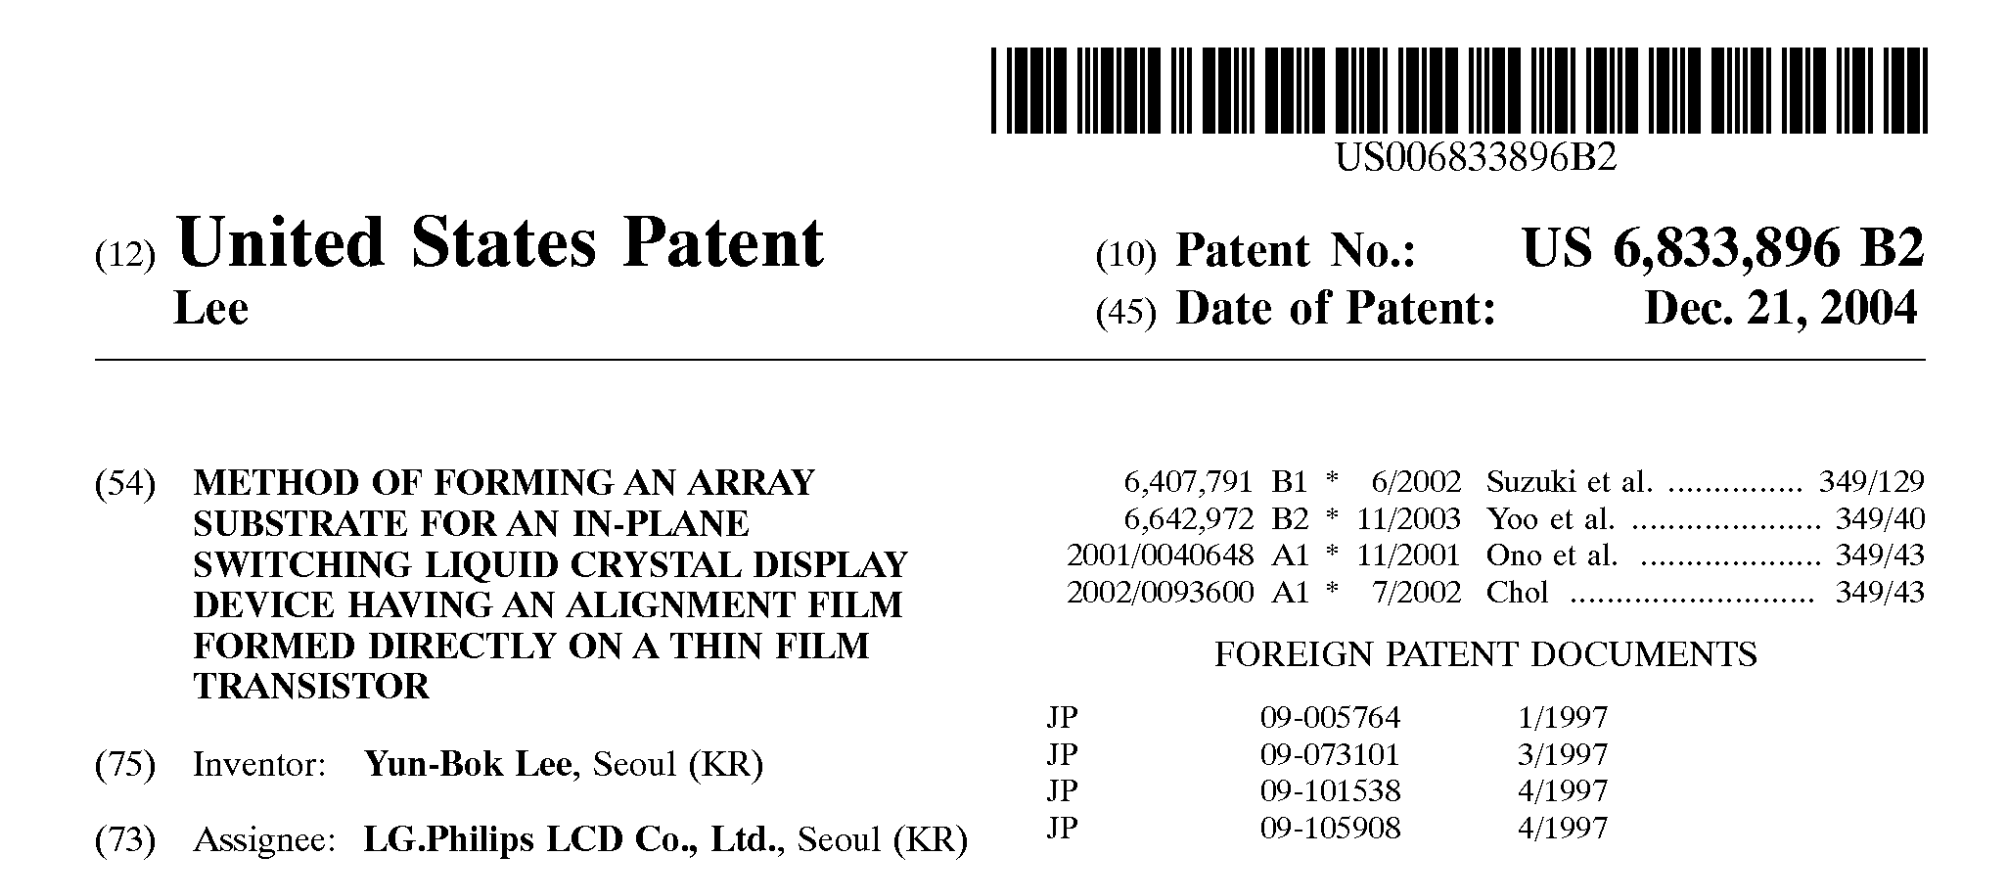
\includegraphics[width=0.8\textwidth]{figures/6833896.png}
	\end{center}
	
	\medskip
	\hrule
	
\medskip
	
	\textbf{Technological classes:} 349 (Liquid Crystal Cells, Elements and Systems), 257 (	Active solid-state devices)
	
	\smallskip
	
	\textbf{Prior art keywords (Google Patents):} layer, method, gate, electrode, substrate
	
	\smallskip
	
	\textbf{Most central keywords (our method):} substrat, semiconductor, insul, gate, transistor
		
	
\end{frame}


\section{Background}

%\begin{frame}{Patent data}
    
%\end{frame}
\begin{frame}{Descriptive statistics}
    % summary of our database ?
    
    % We count 4,666,365 utility patents with an abstract granted from 1976 to 2013. A very small number of patents have a missing abstract, these are patents that have been withdrawn and we do not consider them in the analysis. The number of patents granted each year increases from around 70,000 in 1976 to about 278,000 in 2013. When distributed by the year of application, the picture is slightly different. The number of patents steadily increase from 1976 to 2000 and remains constant around 200,000 per year from 2000 to 2007. Restricting our sample to patent with application date ranging from 1976 to 2007, we are left with 3,949,615 patents. These patents cite 38,756,292 other patents with the empirical lag distribution that has been extensively analyzed in [4]. Conditioned on being cited at least once, a patent receives on average 13.5 citations within a five-year window. 270,877 patents receive no citation during the next five years following application, 10% of patents receive only one citation and 1% of them receive more than 100 citations. A within class citation is defined as a citation between two patents sharing at least one common technological class. Following this definition, 84% of the citations are within class citations. 14% of the citations are between two patents that share the exact same set of technological classes.
    
    \textit{Summary statistics for the USPTO database between 1976 and 2013}
    
    \begin{itemize}
        \item 4,666,365 utility patents from 1976 to 2013
        \item 70,000 in 1976 to 278,000 in 2013
        \item 38,756,292 citation links (84\% of within-class citations)
        \item 270,877 patents with no citations 5 years next to publication
    \end{itemize}
    
    Does this mean that innovation is 4 time larger en 2013 than in 1976... \alert{Not necessary}. Although definitely more specialized.
\end{frame}
\begin{frame}{Number of inventors}
    \begin{figure}
        \centering
        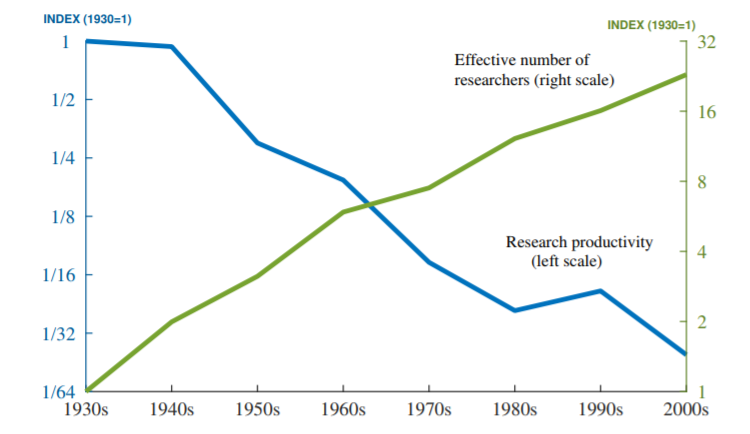
\includegraphics[width=0.8\linewidth]{figures/inventors.png}
        \caption{Evolution of number of researchers and productivity of R\&D. Source: Bloom et al. (2017)}
    \end{figure}
\end{frame}
\begin{frame}{Inventors per patent}
    \begin{figure}
        \centering
        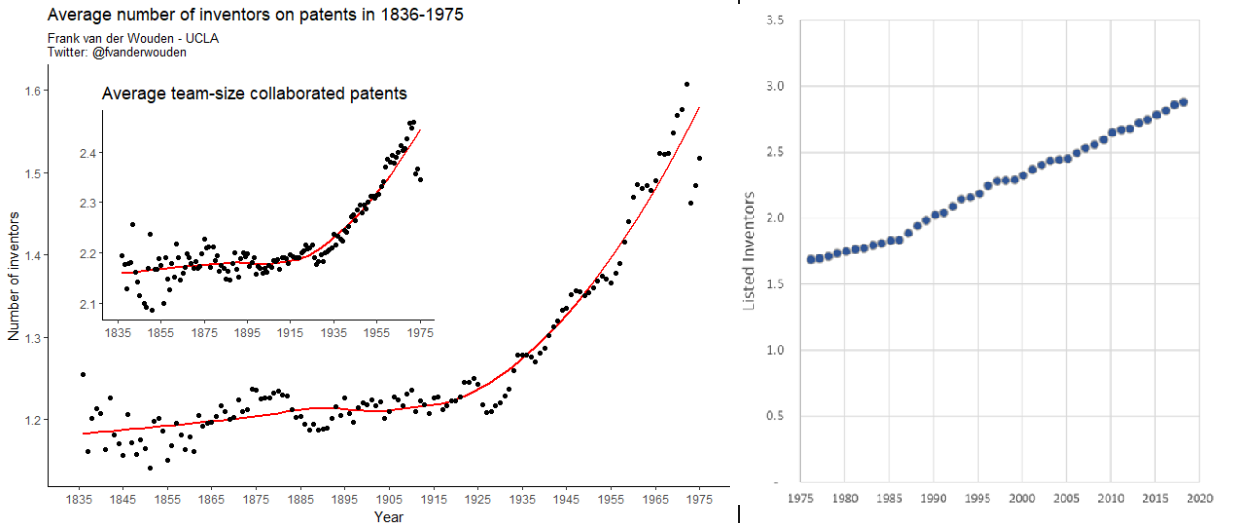
\includegraphics[width=0.8\linewidth]{figures/inv_per_patent.png}
        \caption{Average number of inventors per patent. Source: USPTO.}
    \end{figure}
    
    (It was 1.2 in 1900). Ideas are getting harder to find?
\end{frame}
    
\begin{frame}{Database construction}
    
Construction of a Database from US Patent and Trademark Office redbook 1976-2012 (full patent description), which provide raw data but on separate files and different formats

\bigskip

\textbf{Data Collection Procedure}

\begin{itemize}
\item Automatic download of raw data file
\item Parsing depending on format : \texttt{dat} or \texttt{xml} (varying schema)
\item Uniformisation and storing in MongoDB
\end{itemize}

\bigskip

$\rightarrow$ 4,666,365 patents with text data (abstract); dated by application date (current state of knowledge, differs from the granted date which implies review processes and an exogenous intervention)

\end{frame}
\section{Methods}
\begin{frame}{Extracting relevant n-grams}
    
    % Situate regarding other classical approaches : LDA etc
    
    \textit{Text-mining in python with \texttt{nltk}~\cite{bird2006nltk}}, method adapted from
\cite{chavalarias2013phylomemetic}. Advantage over LDA: scalability and flexibility

   

\bigskip

\begin{itemize}
\item Parsing and tokenizing / pos-tagging (word functions) / stemming  with \texttt{nltk}
\item Selection of potential \textit{n-grams} (with $1 \leq n \leq 3$) with the rule $\bigcap \{NN \cup VBG \cup JJ \}$
%\item Database insertion for instantaneous use (several days $\rightarrow$ 1min)
\item Estimation of \textit{n-grams} relevance, following co-occurrences statistical distribution (\textit{termhood} score as chi-2 score), filtering on relevance to construct co-occurence network
\item Filtering of network edge (parameter $\theta_w$), with an additional exogenous control by technological class keyword concentration to filter nodes (parameter $\theta_c$)
\end{itemize}
\end{frame}


\section{Results}
\begin{frame}{Optimizing network structure}
    
    \centering
    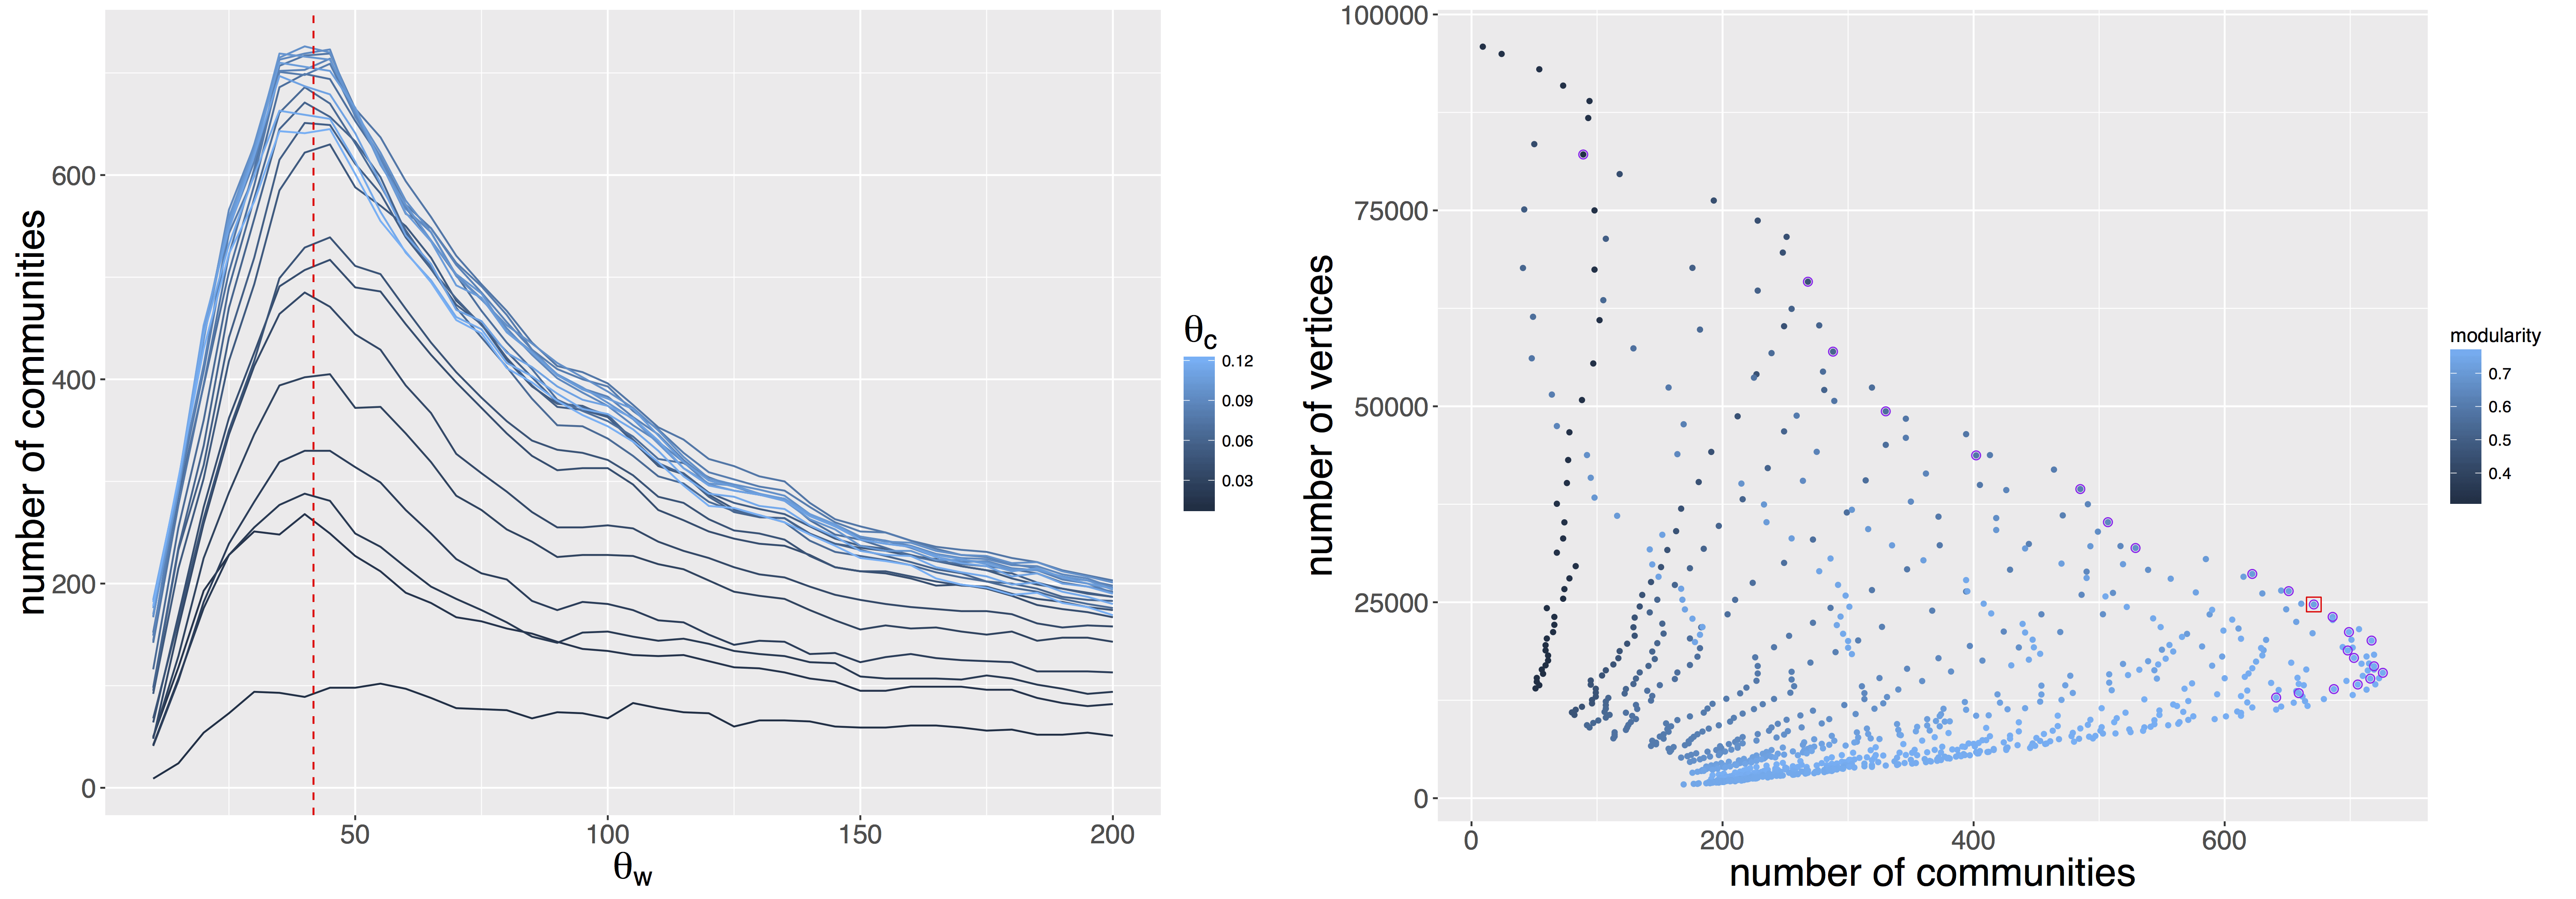
\includegraphics[width=\textwidth]{figures/Fig1.png}
    
    \medskip
    
    \textit{Pareto optimization on cutoff parameters with the objectives of modularity, size and number of communities}
    
\end{frame}

\begin{frame}{Semantic network visualization (example for 2000-2004)}
% TODO check date and parameters
   \centering
    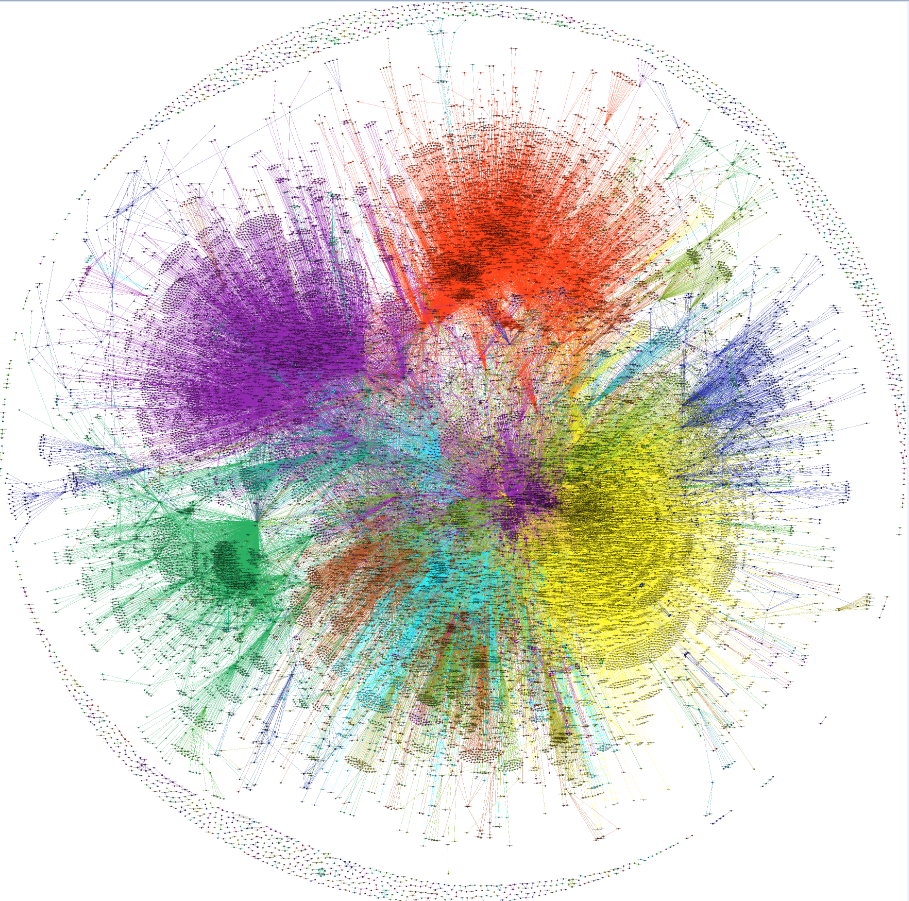
\includegraphics[height=0.85\textheight]{figures/Fig2.png}
    
\end{frame}


\begin{frame}{Classes Examples (2000-2004)}

% discuss on naming class here

\begin{itemize}
\item Memory devices : \texttt{semiconductor memori devic; memori cell plural; memori cell transistor; layer ferroelectr}
\item Chemical analysis : \texttt{time-of-flight mass spectromet; chromatograph column; ion trap mass}
\item Particular steel : \texttt{martensit; austenit stainless steel}
\item Laser : \texttt{emit laser beam; vertic caviti surfac; vcsel}
\item Sewing : \texttt{circular knit machin; stitch; sew machin; embroideri}
\item Lithography : \texttt{lithograph mask; project beam radiat; heat-sensit; planograph print plate}
\item Tobacco : \texttt{cigarett filter; cigarett pack; tobacco; tobacco rod}
\end{itemize}
 \end{frame}



\begin{frame}{Hierarchical class structure}
   \centering
    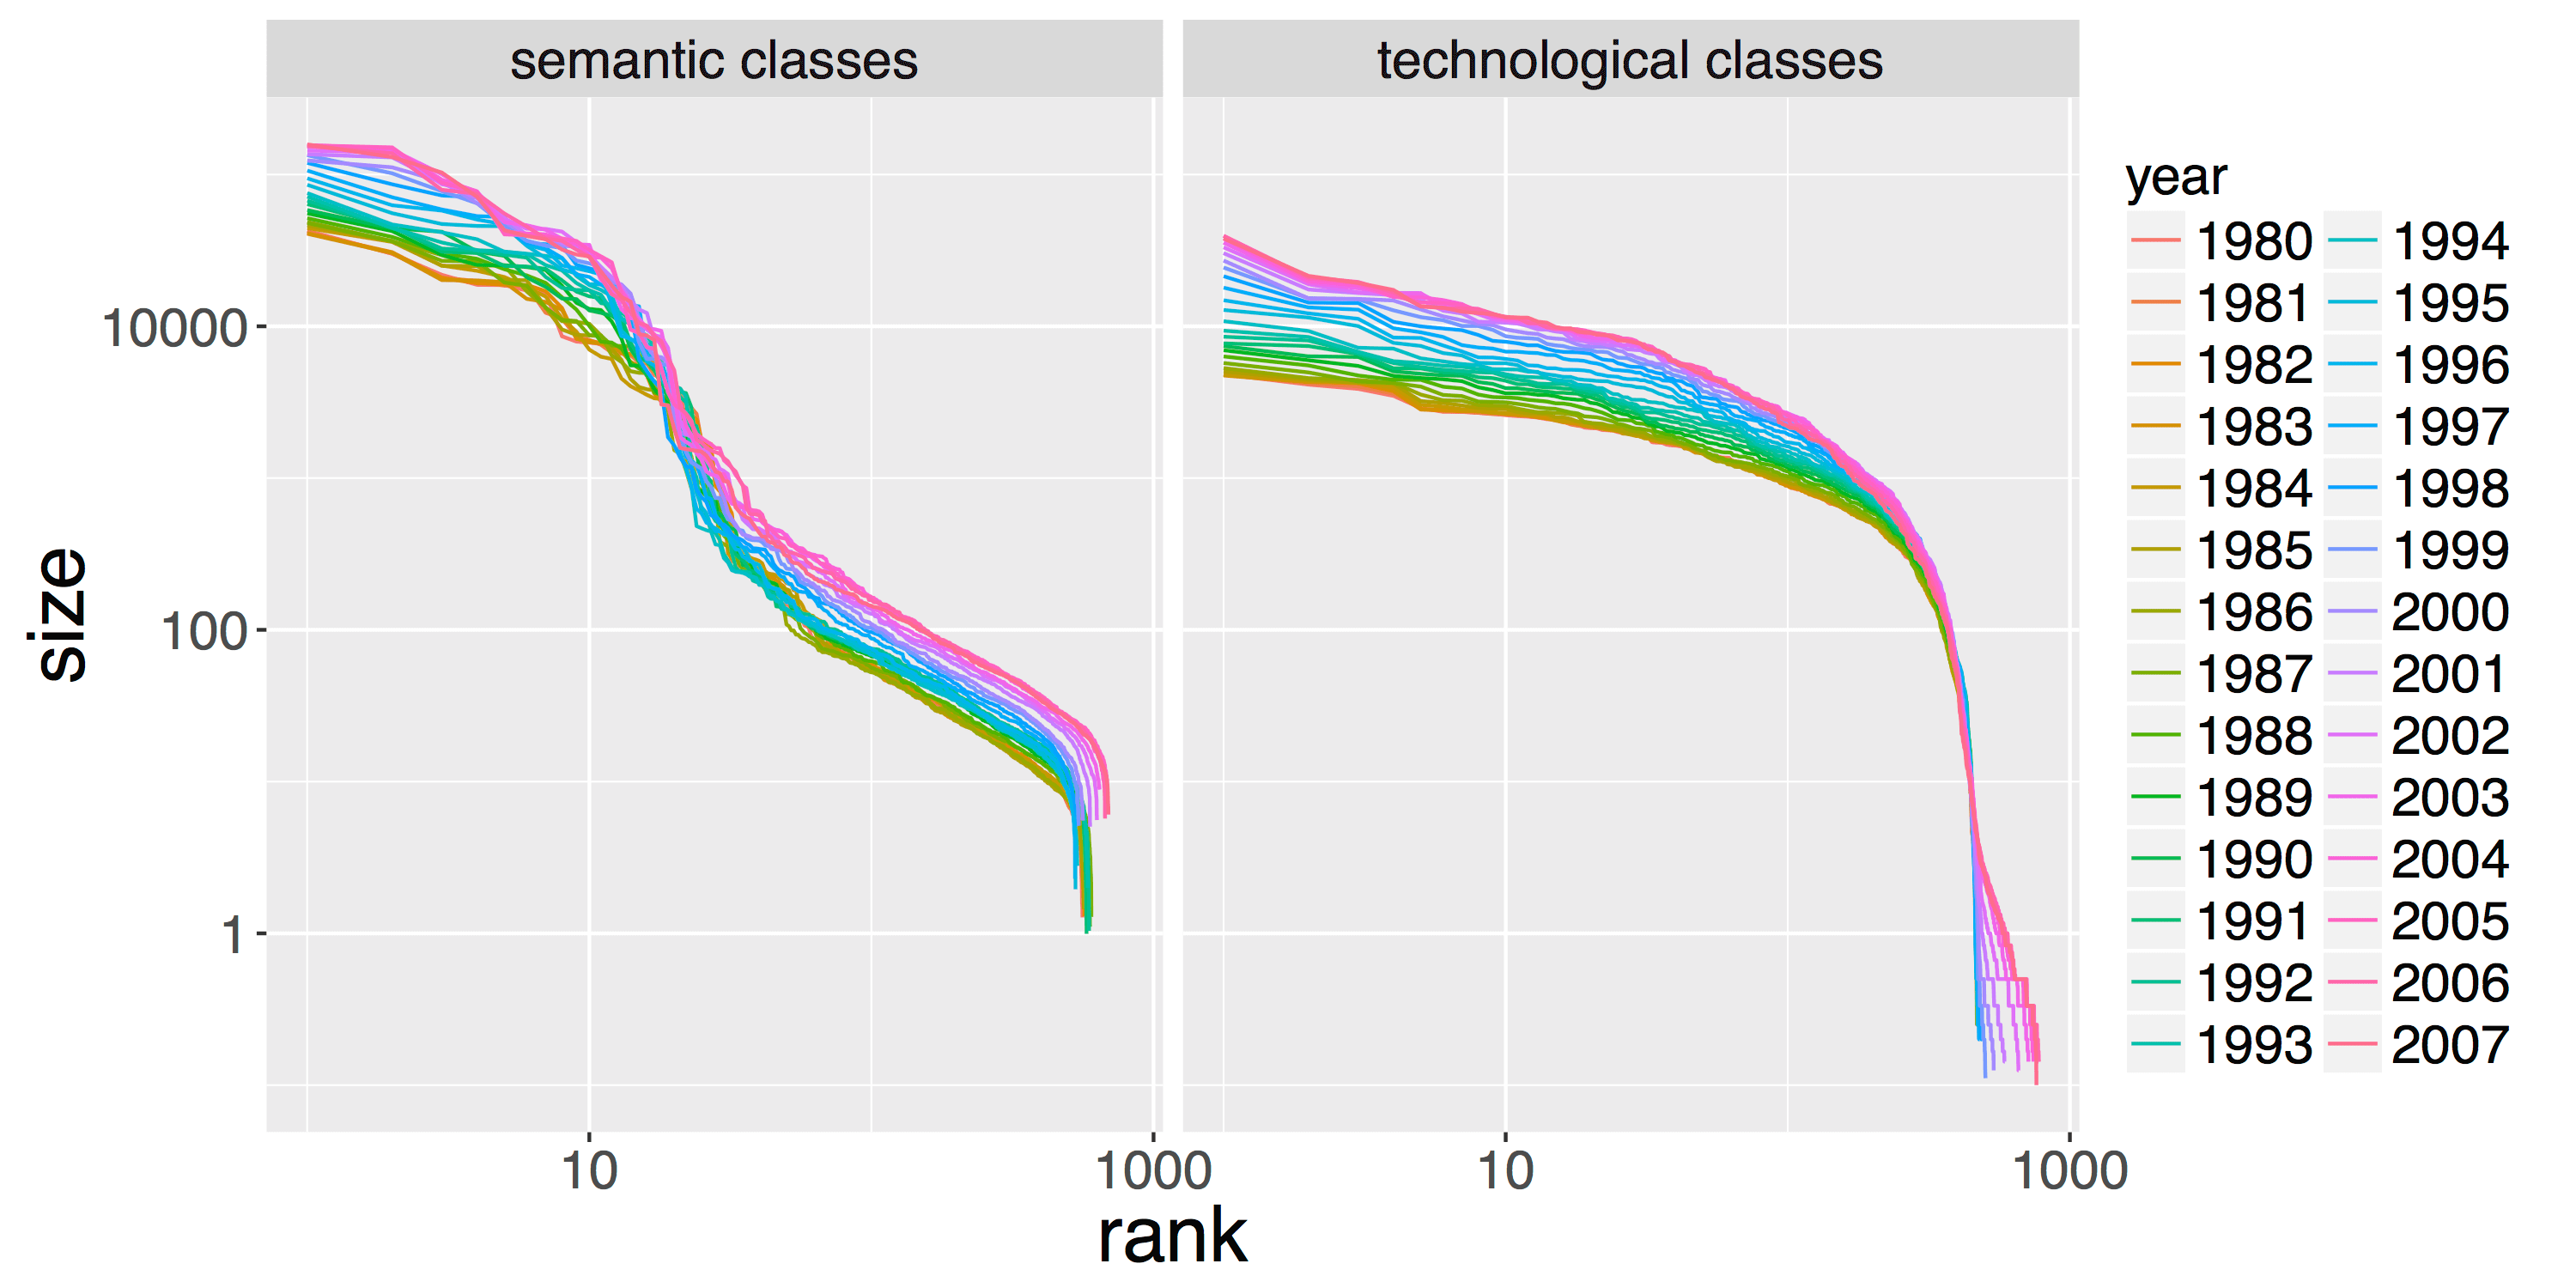
\includegraphics[width=\textwidth]{figures/Fig4.png}
    
    \medskip

    \textit{Fat-tail distribution of class size for both classification, closer to a power-law for semantic classes}
    % different distribution shapes but comparable in order of magnitudes for both extremities -> important for the statistical analysis (?)
    
\end{frame}

\begin{frame}{Evolution of patent diversities}

\label{slide:diversity}
\hyperlink{slide:measures}{\beamerbutton{Back}}

   \centering
    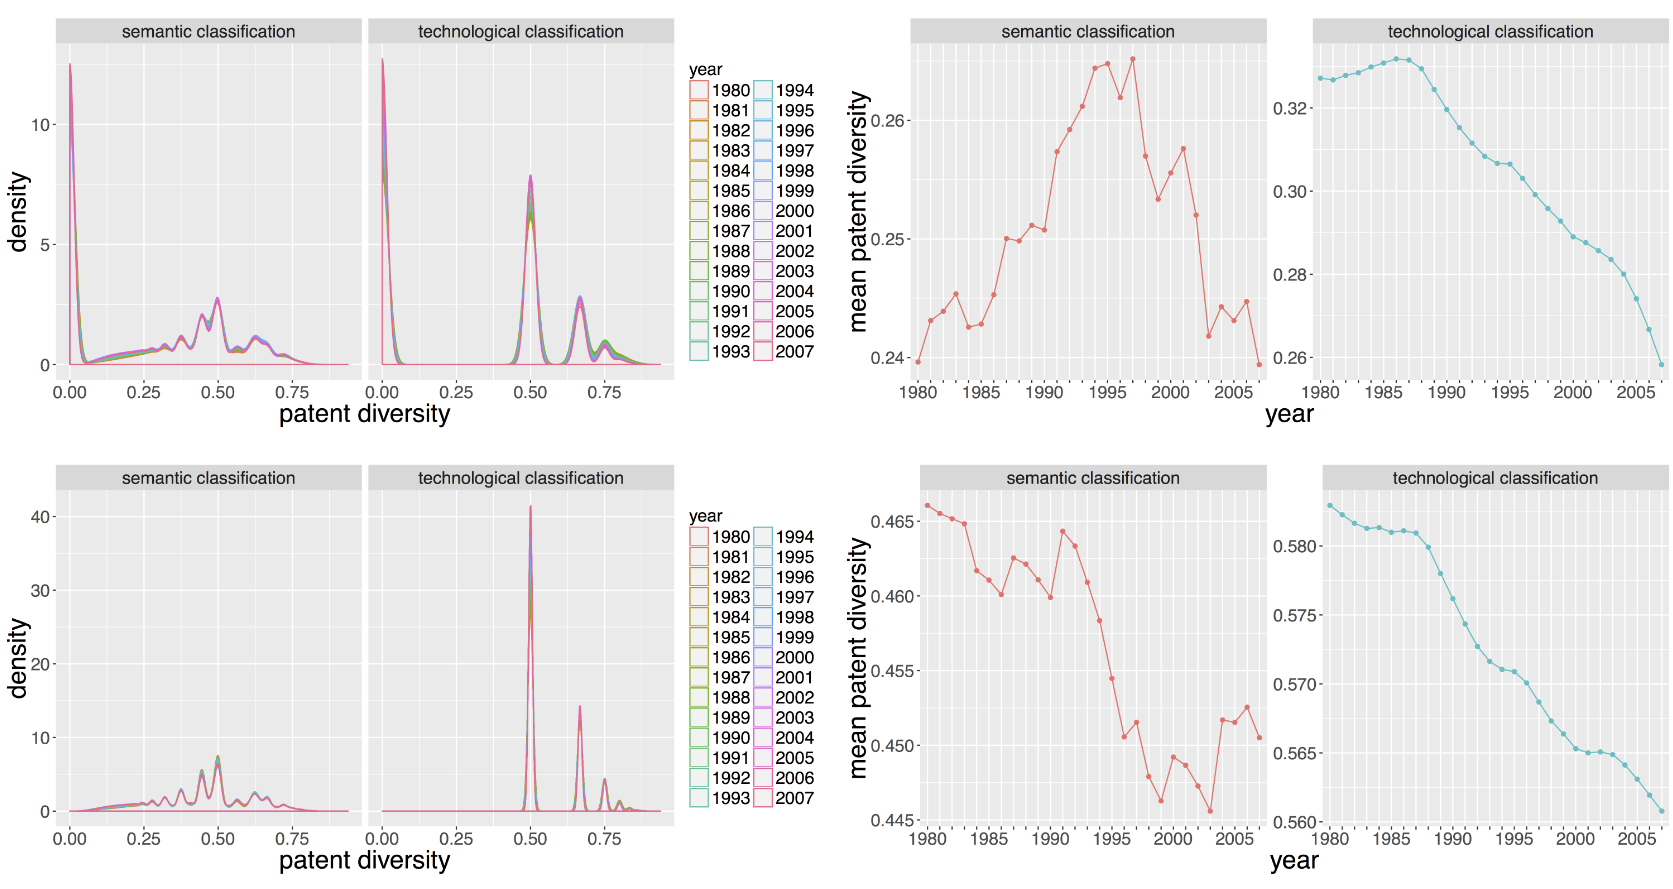
\includegraphics[width=\textwidth]{figures/Fig5.png}
    
    \medskip

    \textit{General increase in average invention specialization seen both for semantic and technological; semantic regime shift in 1996} 
    % "change in the regime of specialization, the new regime being caused by more single-class patents" => confirms the idea of a new type of more specialized inventions
    
\end{frame}

\begin{frame}{Interaction between classes: intra-classification overlaps}
   \centering
    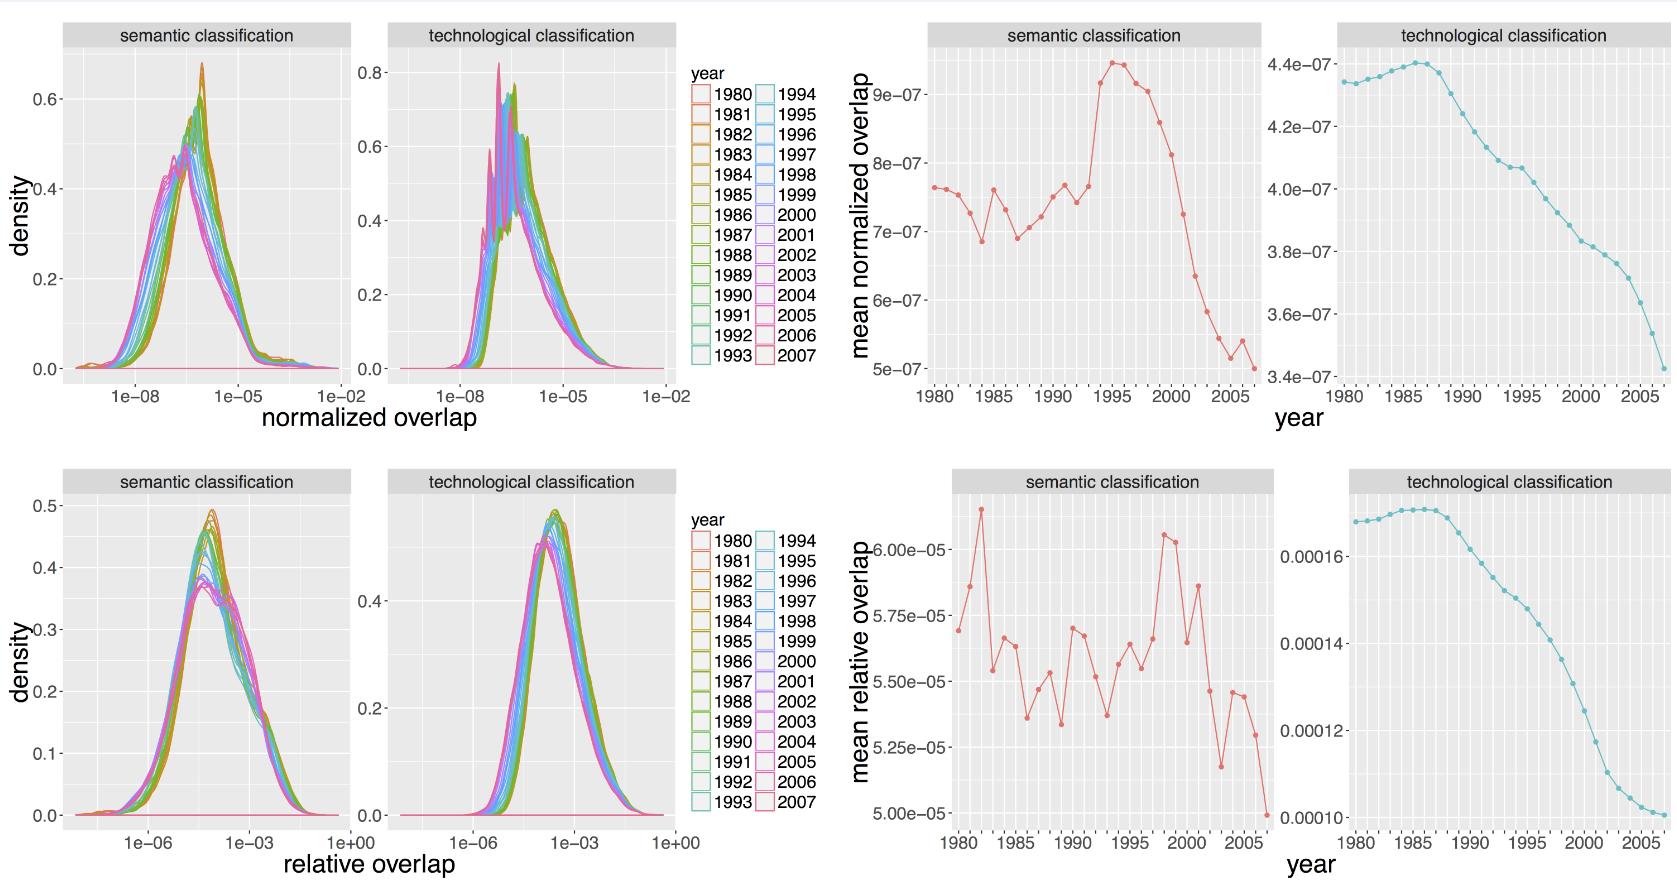
\includegraphics[width=\textwidth]{figures/Fig7.png}
    
    \medskip

    % techno : increasing specializatino trend
    % semantic : consistent with 1996 breakpoint in the structure of technologies - rq : how to control specifically that it is not an artifact of the method / or biased by sizes ?
    
    \textit{Increased technological specialization; qualitative regime shift confirmed in 1996 for the semantic classification}
    
    % discussion on the fact that techno has been done a posteriori ? (for one part at least)
    
\end{frame}

\begin{frame}{Inter-classification overlaps}
   \centering
    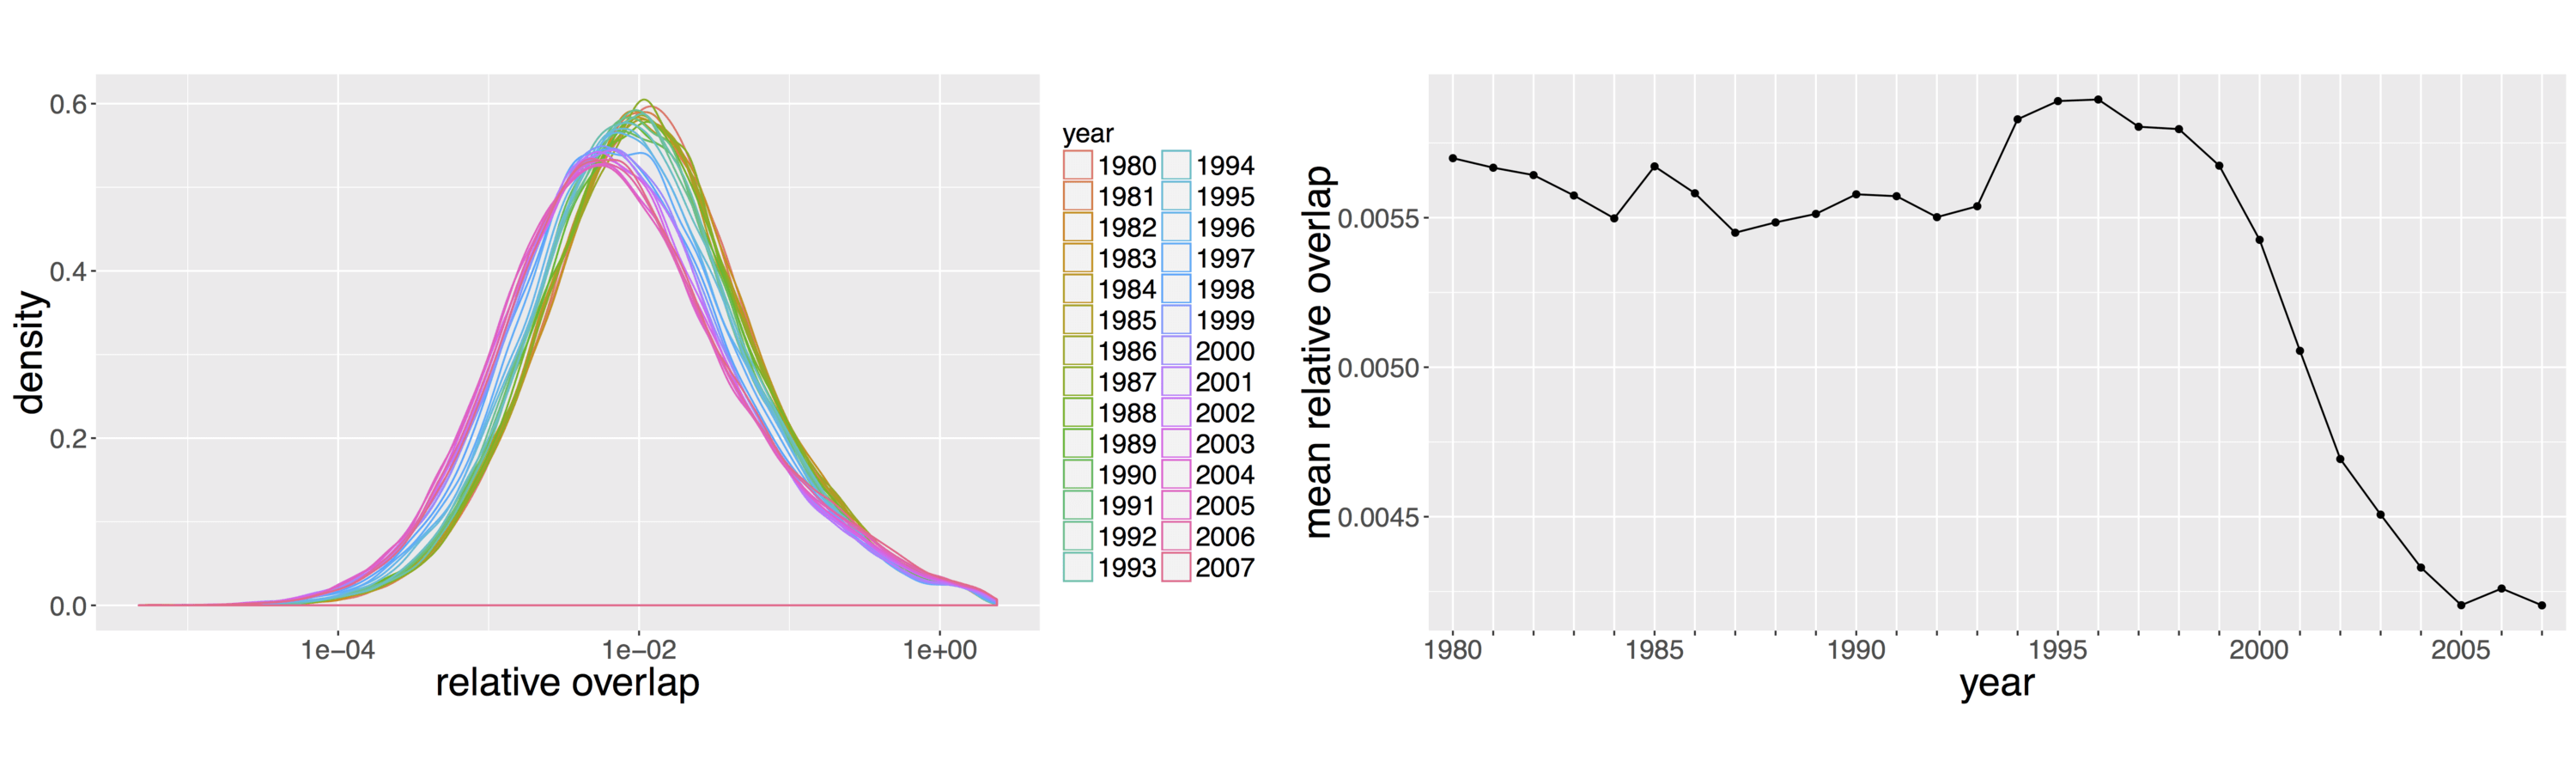
\includegraphics[width=\textwidth]{figures/Fig8.png}
    
    \medskip

    \textit{Constant then decreasing average overlap between technological and semantic classes; confirms the change in nature of inventions around 1996.} 
    
    \smallskip
    
    $\rightarrow$ an impact of new information technologies (regarding knowledge production: from expert and contextualized to automatized search in references e.g.) ? Linked to structural changes in economy (increase in firm concentration since 90s) ?
    
\end{frame}

\begin{frame}{Modularity of classifications} \label{slide:modularity}
\hyperlink{slide:modularity_def}{\beamerbutton{Definition}}

   \centering
    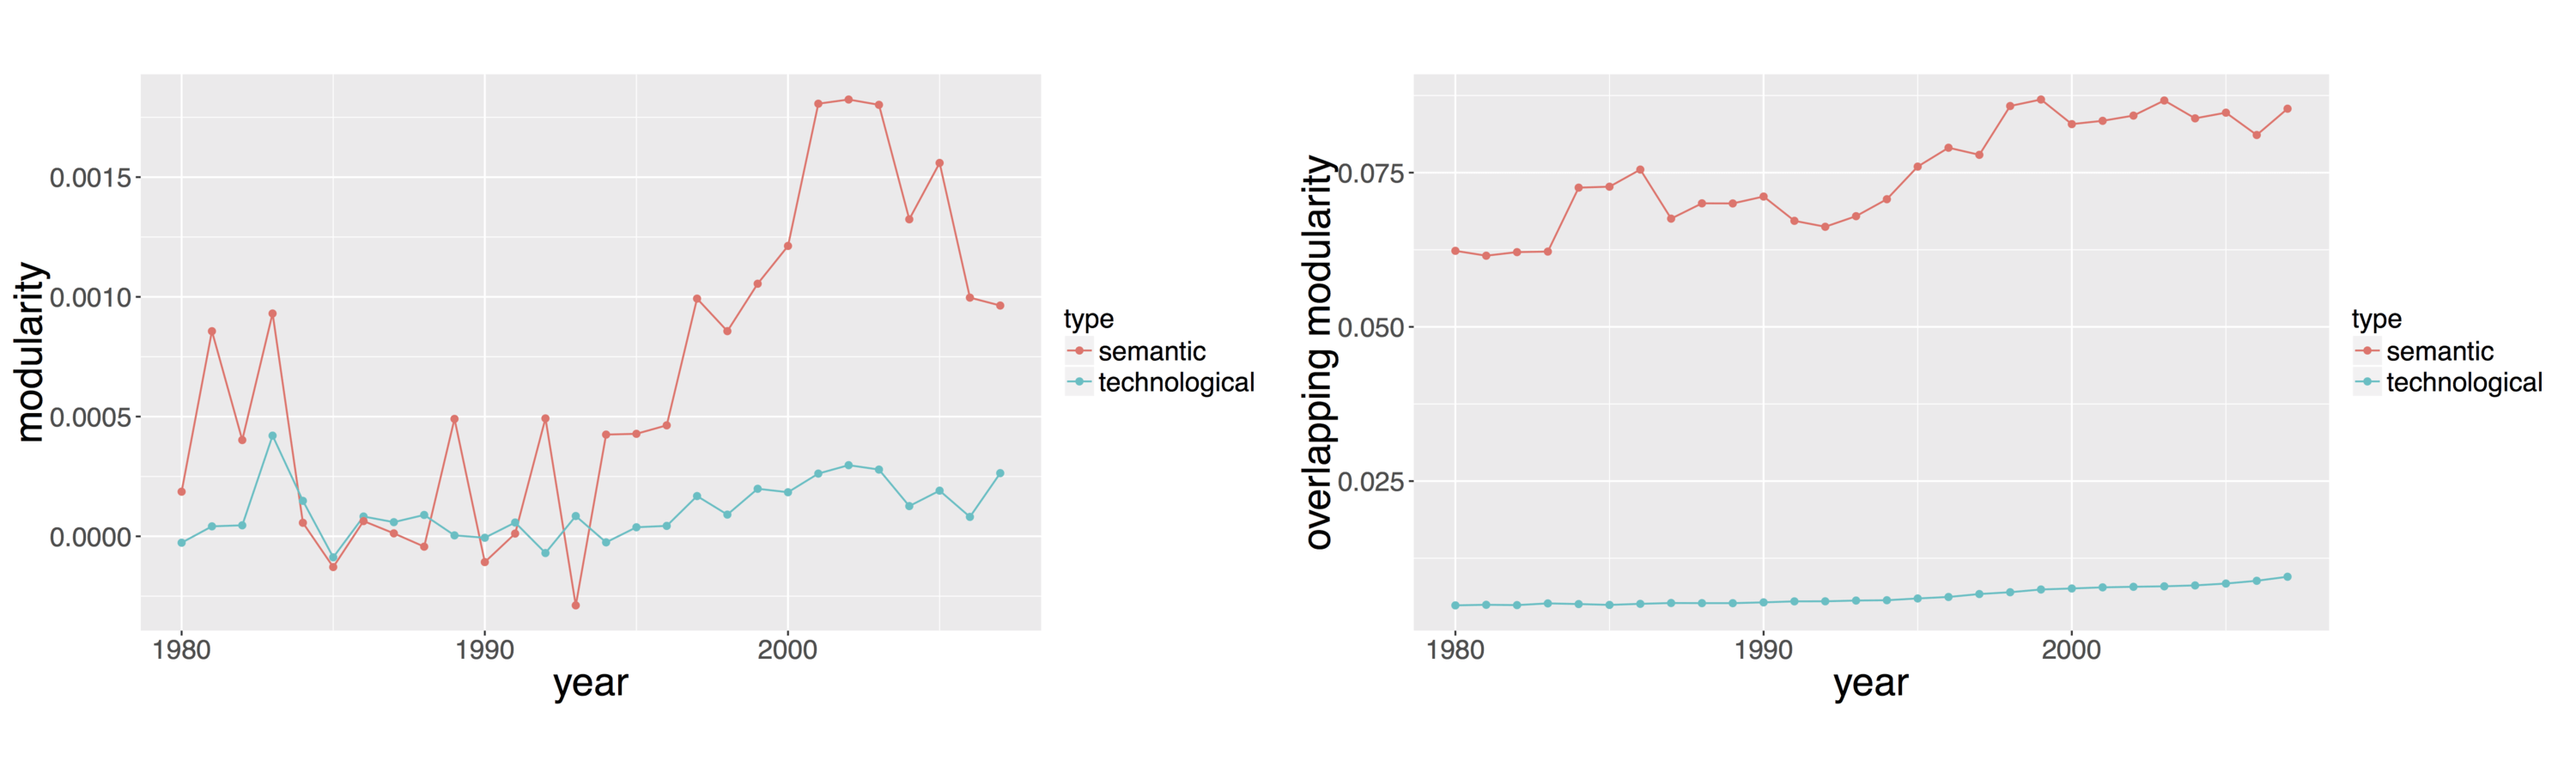
\includegraphics[width=\textwidth]{figures/Fig9.png}
    
    \medskip
    
    \textit{Semantic classification is more significant regarding the structure of the citation network, both for single-class and multi-class modularities (confirmed statistically using a simple Stochastic Block Model).}
    
\end{frame}




\begin{frame}{Summary of outcomes}
    \begin{itemize}
        \item A clean redbook
        \item Semantic and technological classification for each patent
        \item Network based measure of centrality for each patent
    \end{itemize}
    
    Most importance insight: semantic classification does carry some information beyond what the technological classification provides.
\end{frame}


\section{Conclusion}
\begin{frame}{Possible developments}
\textbf{Direct}
    \begin{itemize}
        \item Look at the correlation between patent quality indicators and centrality indices.
        \item Use patent-firm matching to study a \emph{firm-level} semantic network.
        \item Extending the analysis to other patent offices (EPO/JPO).
    \end{itemize}
    \pause
\textbf{Economic}
    \begin{itemize}
        \item Linking semantic measures to values of firms
        \item Can semantic proximity helps understand M\&A?
        \item Firms trajectories in relation to their life-cycle
    \end{itemize}
    \pause
\textbf{Technology}
\begin{itemize}
    \item Measure of complementarity between technology?
    \item Possible application to detection of emerging research fronts
    \item An interactive exploration of semantic content?
\end{itemize}
\end{frame}
\begin{frame}{Other projects}
     
     \textbf{At the interface of geography and economics}
     
     \smallskip
     
     $\rightarrow$ Quantifying the diffusion of innovation in urban systems, and its co-evolution with the socio-economic structure
     
     \smallskip
     
     \bigskip
     
     \textbf{Possible developments in other disciplines}
     
      \smallskip
     
     $\rightarrow$ Agent-based modeling of interactions between technologies
     
     \smallskip
     
     $\rightarrow$ Full-text mining and history of technology \\

\end{frame}

\begin{frame}{Conclusion}

$\rightarrow$ A quantitative epistemology insight into the evolution of technology

\medskip

$\rightarrow$ Towards reflexive approaches in science and technology to ease technological transfer / foster the co-evolution between the two ?


\bigskip

%\bigskip

\textbf{Paper: } Bergeaud, A., Potiron, Y., \& Raimbault, J. (2017). Classifying patents based on their semantic content. PloS one, 12(4), e0176310.

\medskip
\textbf{Open repository} at \texttt{https://github.com/JusteRaimbault/PatentsMining}\\\medskip
\textbf{Raw database} at \texttt{http://dx.doi.org/10.7910/DVN/BW3ACK}\\\medskip 
\textbf{Semantic classification database} at  \texttt{http:// dx.doi.org/10.7910/DVN/ZULMOY}\\\medskip
\textbf{Acknowledgments}: thanks to ISC-PIF for access to the computation infrastructure.

\end{frame}


\begin{frame}{Reserve slides}
    
    \centering
    \Huge
    \textbf{Reserve slides}
    
\end{frame}

\begin{frame}{Previous work on patents and text-mining}

    \begin{itemize}
\item \cite{griliches1998patent}: patent as an economic indicator
\item \cite{Youn:2015fk} interaction between technological fields ; combinatorial nature of inventions
\item \cite{2016arXiv160207928B} citation network analysis to detect emerging research front
\item \cite{gerken2012new} \cite{tseng2007text} semantic analysis (remains limited to specific fields and time windows)
\end{itemize} 

\end{frame}



\begin{frame}{Technical aspects}
	
	$\rightarrow$ Temporal complexity: $\mathcal{O}(N_P)$ for keyword extraction and co-occurrences (constant $l_{max}^2$); parallelization on a 60 cores server for a ``reasonable'' computation time. 
	
	\bigskip
	
	$\rightarrow$ Memory complexity: co-occurrence matrices in $\mathcal{O}(K_W^2)$; necessitates around 600Go RAM when parallelized. 
	
	\bigskip

	$\rightarrow$ Database management: MongoDB (nosql suited to big data).	
	
	
	
	
\end{frame}



\begin{frame}{An application of the method to a scientific corpus}
	 % illustration de la flexibilite de la methode
	 
	 
	 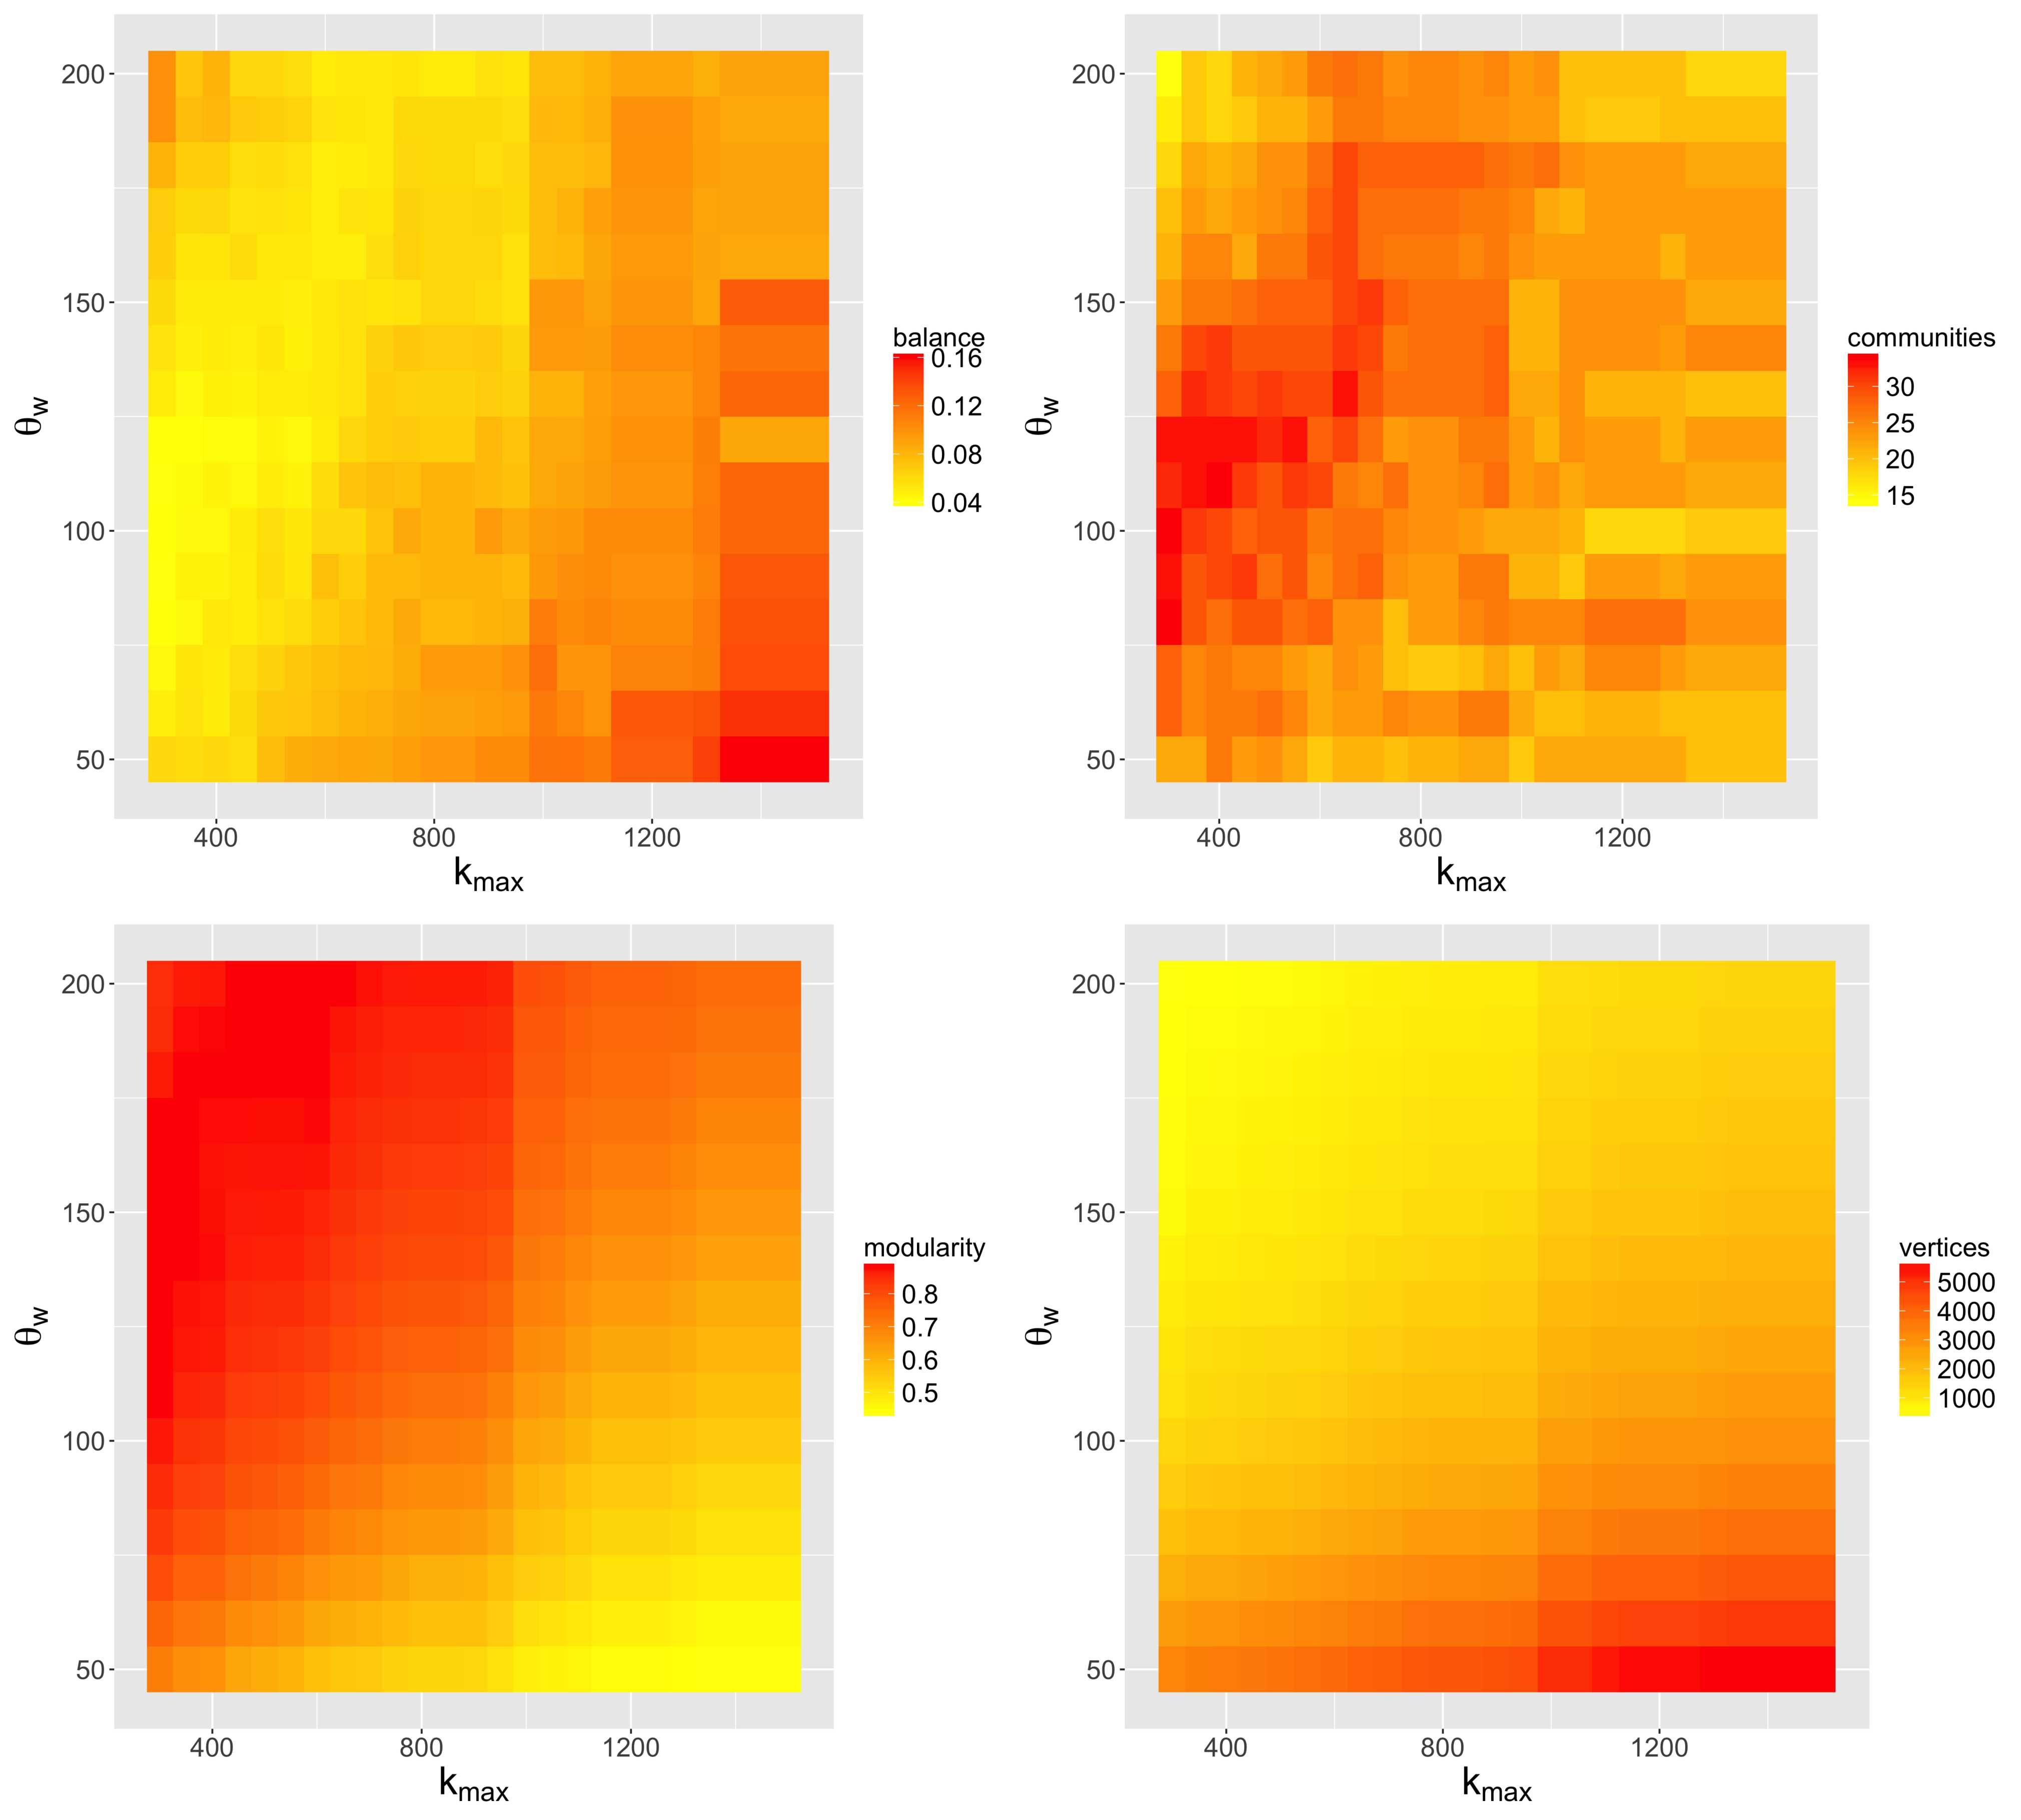
\includegraphics[width=0.49\textwidth]{figures/cyb_Fig6.jpg}
	 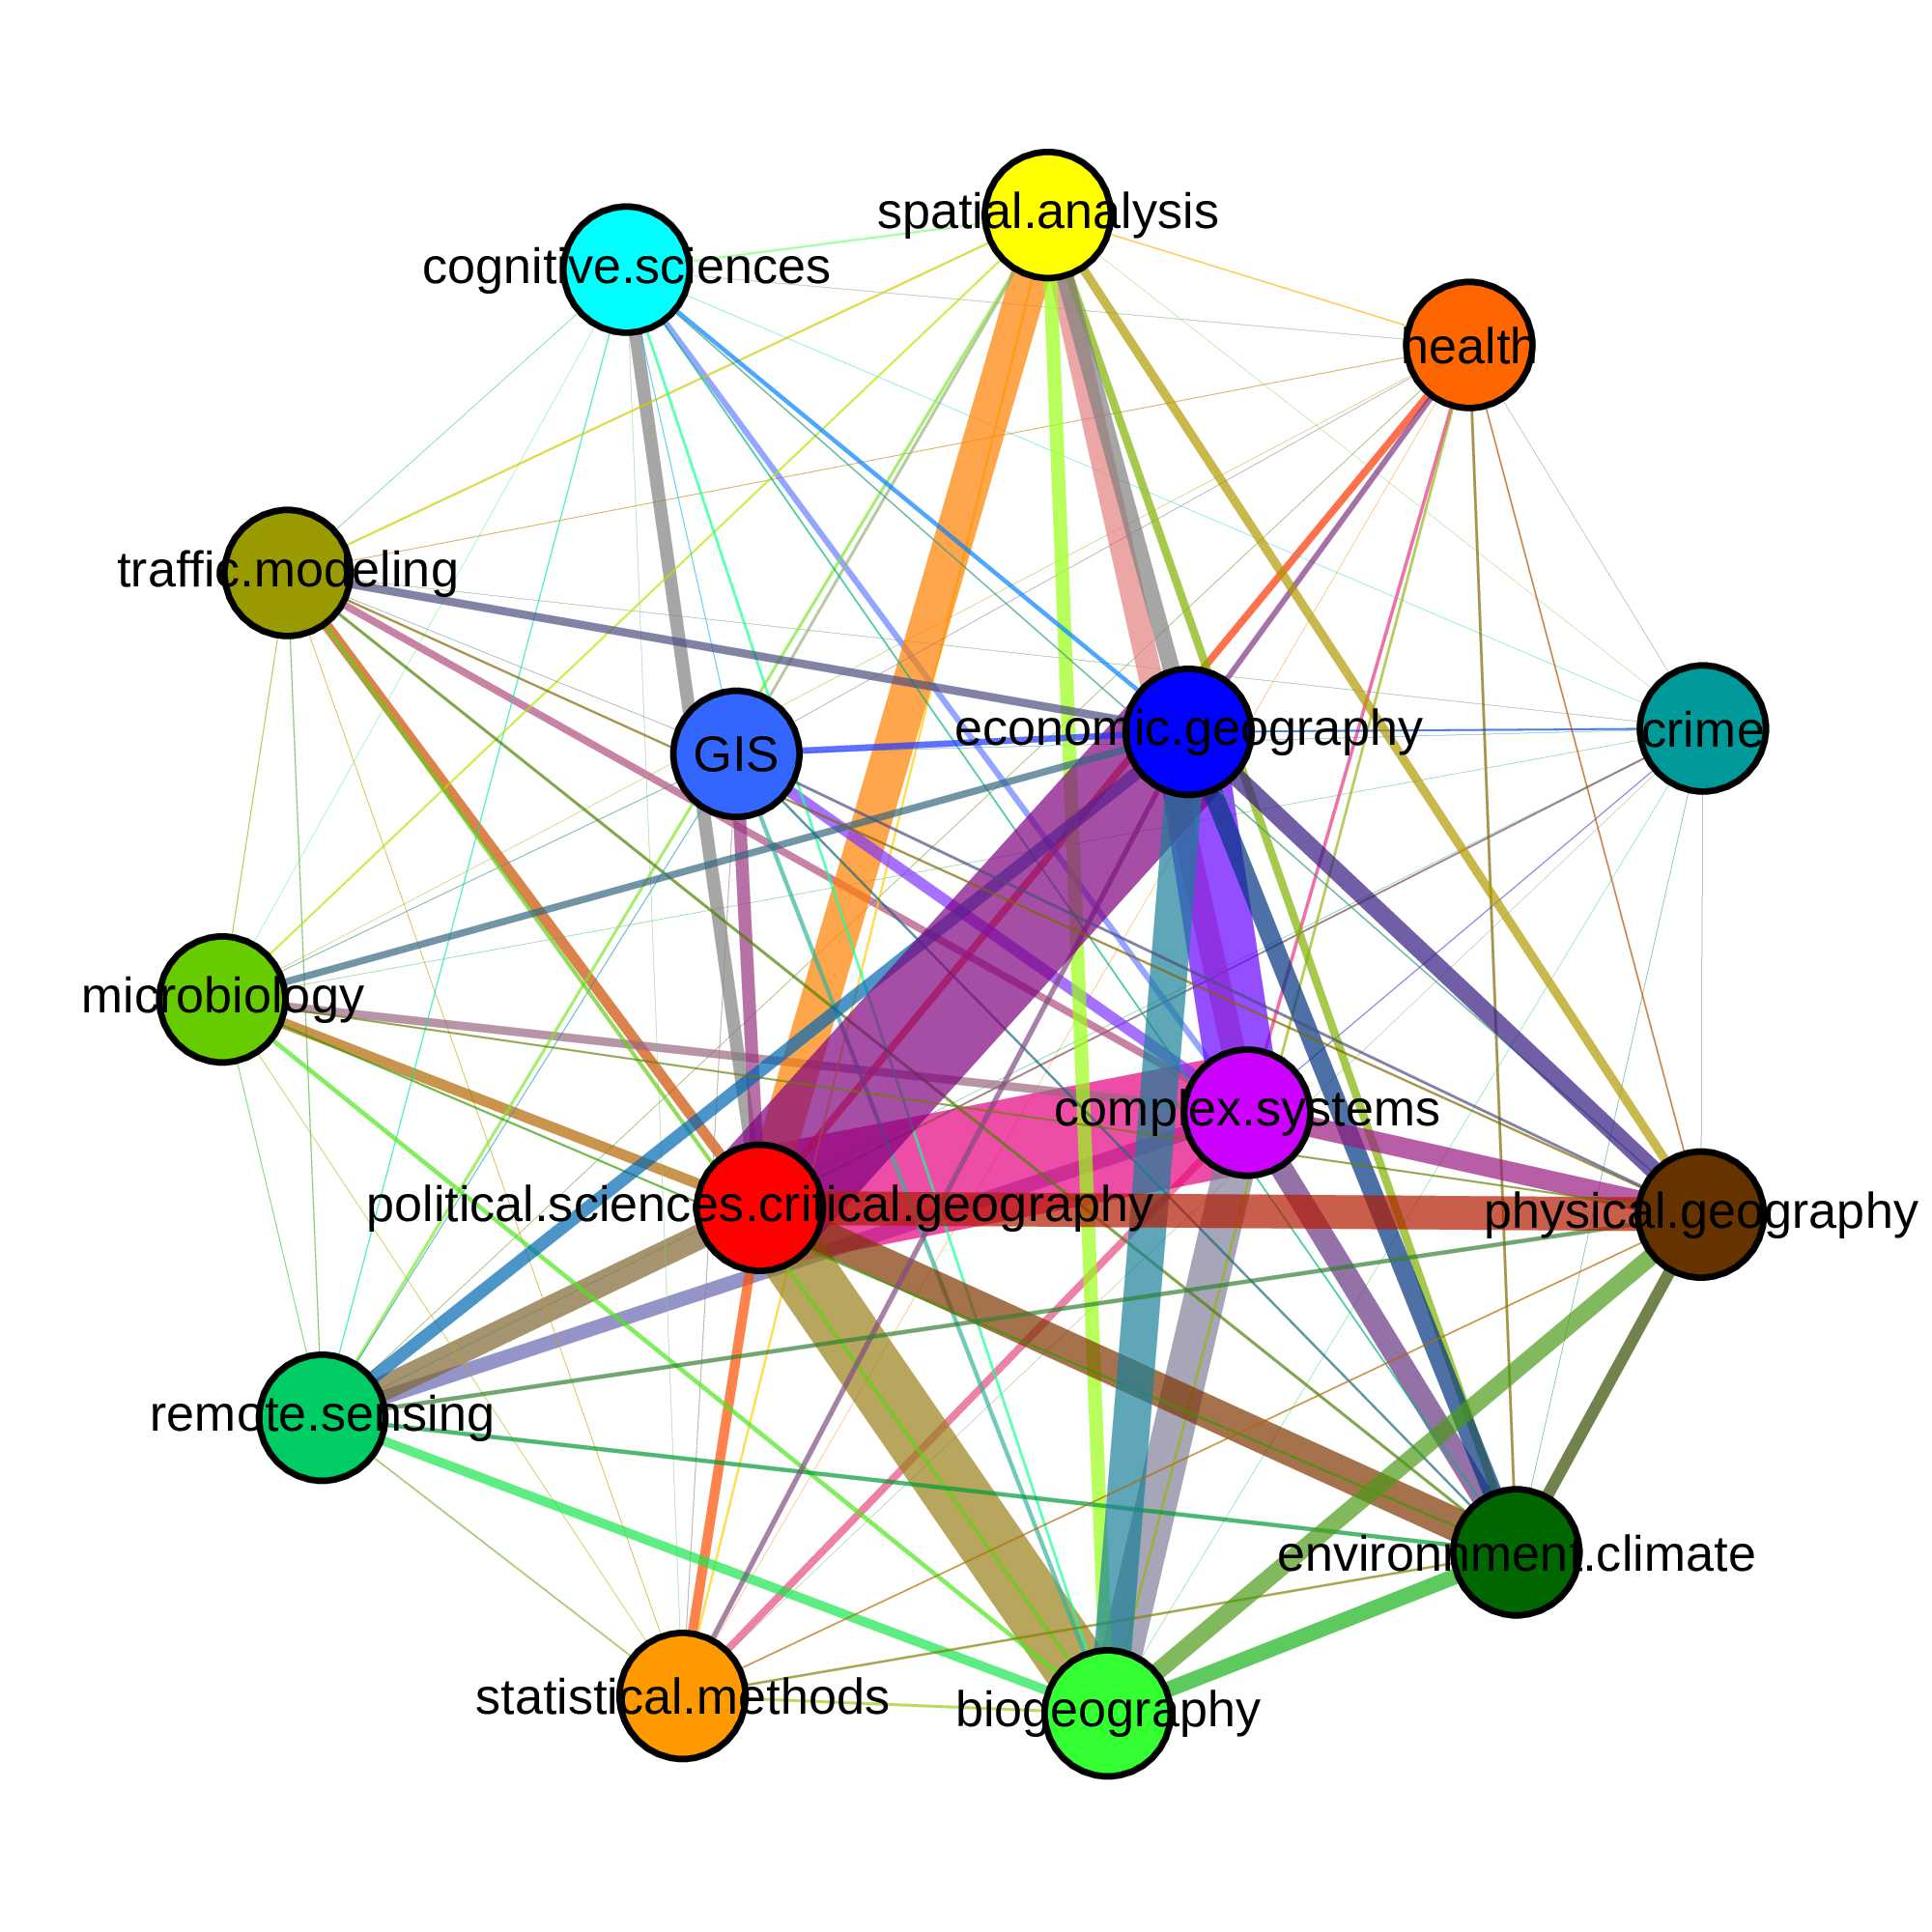
\includegraphics[width=0.49\textwidth]{figures/cyb_Fig8.jpg}
	
	\medskip
	
	\textit{The method has been applied to a scientific corpus; adaptation of optimization procedures as the topological structure is different.} \cite{raimbault2017exploration}
	
		
\end{frame}





\begin{frame}{Estimation of n-gram relevance}\label{slide:relevance}
    
    \begin{itemize}
        \item Termhood-based selection of a fixed number of keywords $K_W = 100,000$ (\textit{difficulty to select terms in general}) \hyperlink{slide:filtration}{\beamerbutton{Definition}}
        % bias to keep fixed size of vocabulary ?
        %  if variable = f(patents) -> arbitrary fixes a number of kws "per patent"; should them optimize regarding an exogenous criteria, which one ?
        %  if fixed, this number varies, so the resolution of classes varies, thus larger classes more recently ? peak in sizes contradicts that, so should not capture this bias significantly (or structure is more important).
        \item Estimation on temporal moving windows $\left[t - T_w ; t\right]$ (fixed to $T_W = 4y$ after sensitivity analysis)
        \item Filtering of network edge (parameter $\theta_w$), with an additional exogenous control by technological class keyword concentration to filter nodes (parameter $\theta_c$)
        % potential bias here -> would capture the exogenous classification system ? idem our results suggest that bias does not dominate results
        \item Low sensibility to the length of the time window for the network structure  
\hyperlink{slide:sensitivity}{\beamerbutton{Sensitivity analysis}}
% in comparable lengths of course
    \end{itemize}
    
\end{frame}



\begin{frame}{Filtration measures}

\label{slide:filtration}
\hyperlink{slide:relevance}{\beamerbutton{Back}}



    
    \textit{1. Unithood: n-gram specific frequency-based filtration ($4\cdot K_W$ keywords)}
    
	\[
	u_i = f_i\cdot \log{(1 + l_i)}
	\]
    
    \medskip
    
    \textit{2. Termhood: chi-square statistic for the uniformity of co-occurences}
    
    \medskip
    
    \begin{eqnarray}
\label{termhood}
t_i = \sum_{j\neq i}\frac{\left( M_{ij} - \sum_{k}M_{ik} \sum_{k} M_{jk}\right)^2}{\sum_{k}M_{ik} \sum_{k} M_{jk}}.
\end{eqnarray}

    \medskip

	\textit{3. Edge weight filtration with a threshold of $\theta_w = \theta_w^{(0)}\cdot N_P$}
	
	\medskip

	\textit{4. Node filtration with a threshold $\theta_c$ on technological class concentration given by}
    
    \[
    c_{tech}(s) = \displaystyle \sum_{j=1}^{N^{(tec)}} \frac{k_j(s)^2}{ \left(\sum_i k_i(s)\right)^2}
    \]
    
    
\end{frame}

\begin{frame}{Patent measures}
\label{slide:measures}
\hyperlink{slide:diversity}{\beamerbutton{Back}}
    
    \textit{Diversity}
    \[
D_i^{(z)} = 1 - \sum_{j =1}^{N^{(z)}} {p_{ij}^2}, \text{ with } z \in \{tec, sem\}
	\]
    
    \medskip

	\textit{Originality and Generality}

	\[
O_i^{(z)} = \displaystyle 1 - \sum_{j =1}^{N^{(z)}}{\left(\frac{\displaystyle \sum_{i' \in I_i}{p_{i'j}}}{\displaystyle \sum_{k =1}^{N^{(z)}}{\displaystyle \sum_{i' \in I_i}{p_{i'k}}}}\right)^2}
\text{ and } G_i^{(z)} = \displaystyle 1 - \sum_{j =1}^{N^{(z)}}{\left(\frac{\displaystyle \sum_{i' \in \tilde{I}_i}{p_{i'j}}}{\displaystyle \sum_{k =1}^{N^{(z)}}{\displaystyle \sum_{i' \in \tilde{I}_i}{p_{i'k}}}}\right)^2}
\]
    

    
\end{frame}



\begin{frame}{Definition of modularities} \label{slide:modularity_def}
\hyperlink{slide:modularity}{\beamerbutton{Back}}

    Directed simple modularity:
    \[
Q_d^{(z)} = \displaystyle \frac{1}{N_P}\sum_{1\leq i,j\leq N_P}\left[A_{ij} - \frac{k_{i}^{in}k_{j}^{out}}{N_P}\right]\delta(c_i,c_j),
\]

%with $A_{ij}$ the citation adjacency matrix (i.e. $A_{ij} = 1$ if there is a citation from the $i$th patent to the $j$th patent, and $A_{ij}=0$ if not), $k_i^{in}=\left| I_i\right|$ (resp. $k_i^{out}= \left|\tilde{I}_i \right|$) in-degree (resp. out-degree) of patents (i.e. the number of citations made by the $i$th patent to others and the number of citations received by the $i$th patent). $Q_d$ can be defined for each of the two classification systems: $z \in \{tec, sem\}$. If $z=tec$, $c_i$ is defined as the main patent class, which is taken as the first class whereas if $z=sem$, $c_i$ is the class with the largest probability.

\bigskip

Multi-class modularity:

\[
\displaystyle Q_{ov}^{(z)} = \frac{1}{N_P} \sum_{c = 1}^{N^{(z)}} \sum_{1\leq i,j \leq N_P}\left[F(p_{ic},p_{jc})A_{ij} - \frac{\beta_{i,c}^{out}k_i^{out}\beta_{j,c}^{in}k_j^{in}}{N_P}\right],
\]
where
\[
 \beta_{i,c}^{out} =   \frac{1}{N_P} \displaystyle \sum_j F(p_{ic},p_{jc}) \text{ and } \beta_{j,c}^{in} =  \frac{1}{N_P} \displaystyle \sum_i F(p_{ic},p_{jc}).
\]
    
\end{frame}



\begin{frame}{Size of classes}
   \centering
    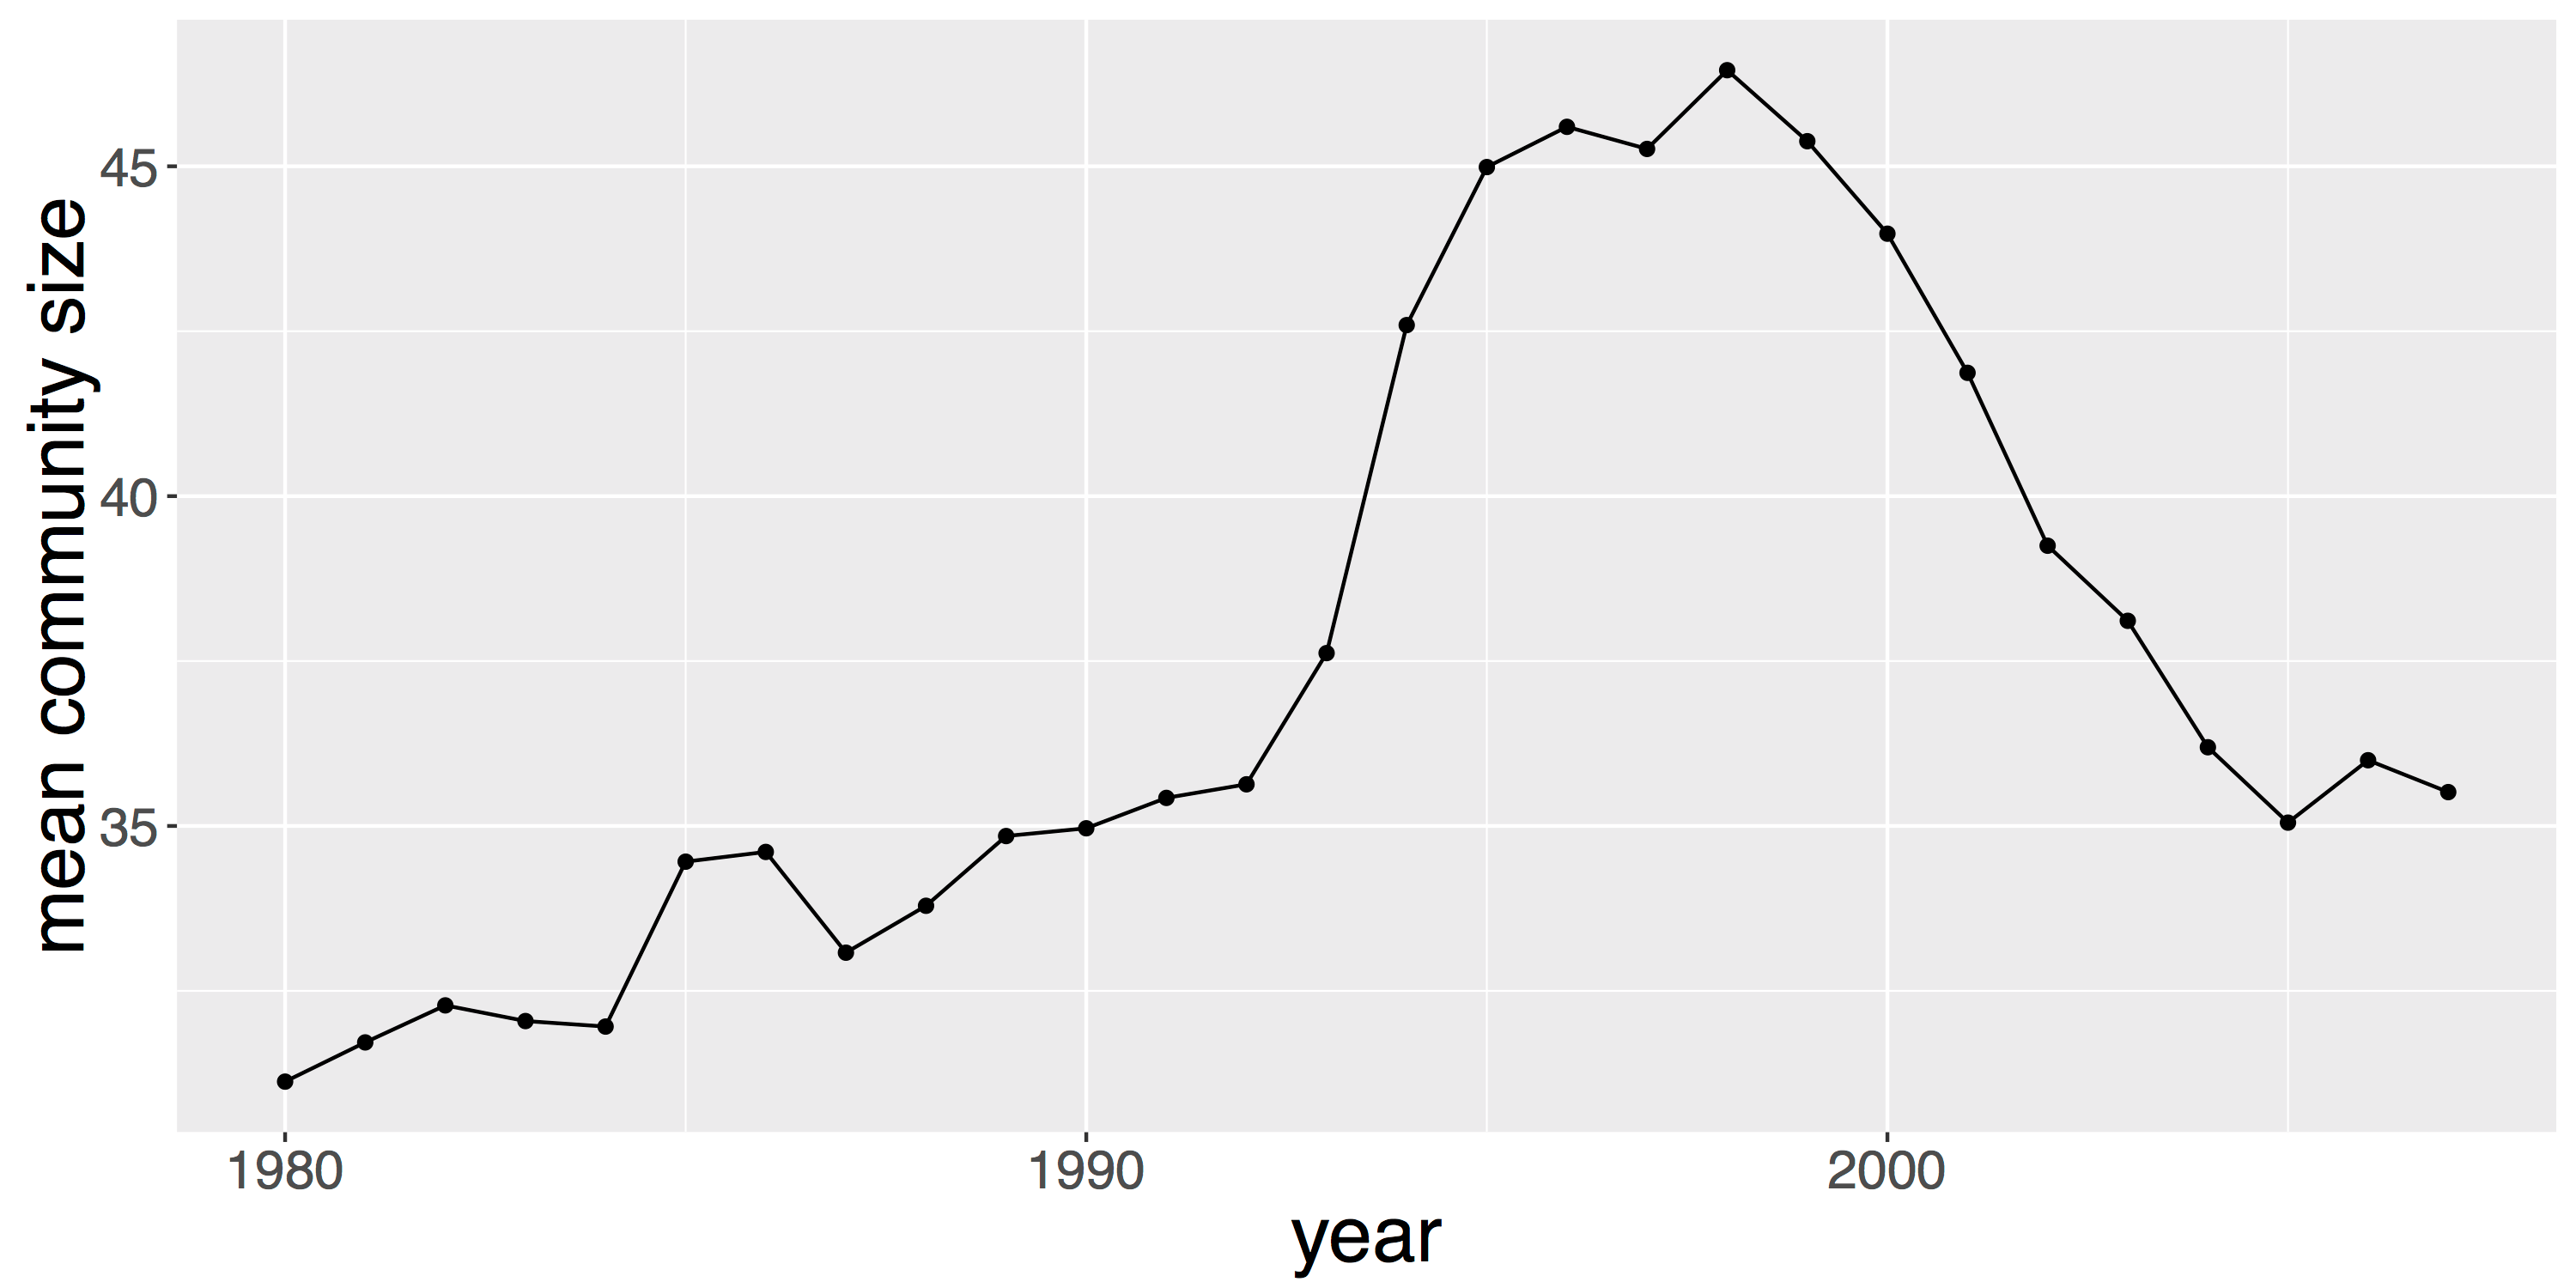
\includegraphics[width=\textwidth]{figures/Fig3.png}
    
    \medskip
    
    \textit{A peak in average class size around 1998}
    
\end{frame}



\begin{frame}{Originality and generality measures}
    \centering
    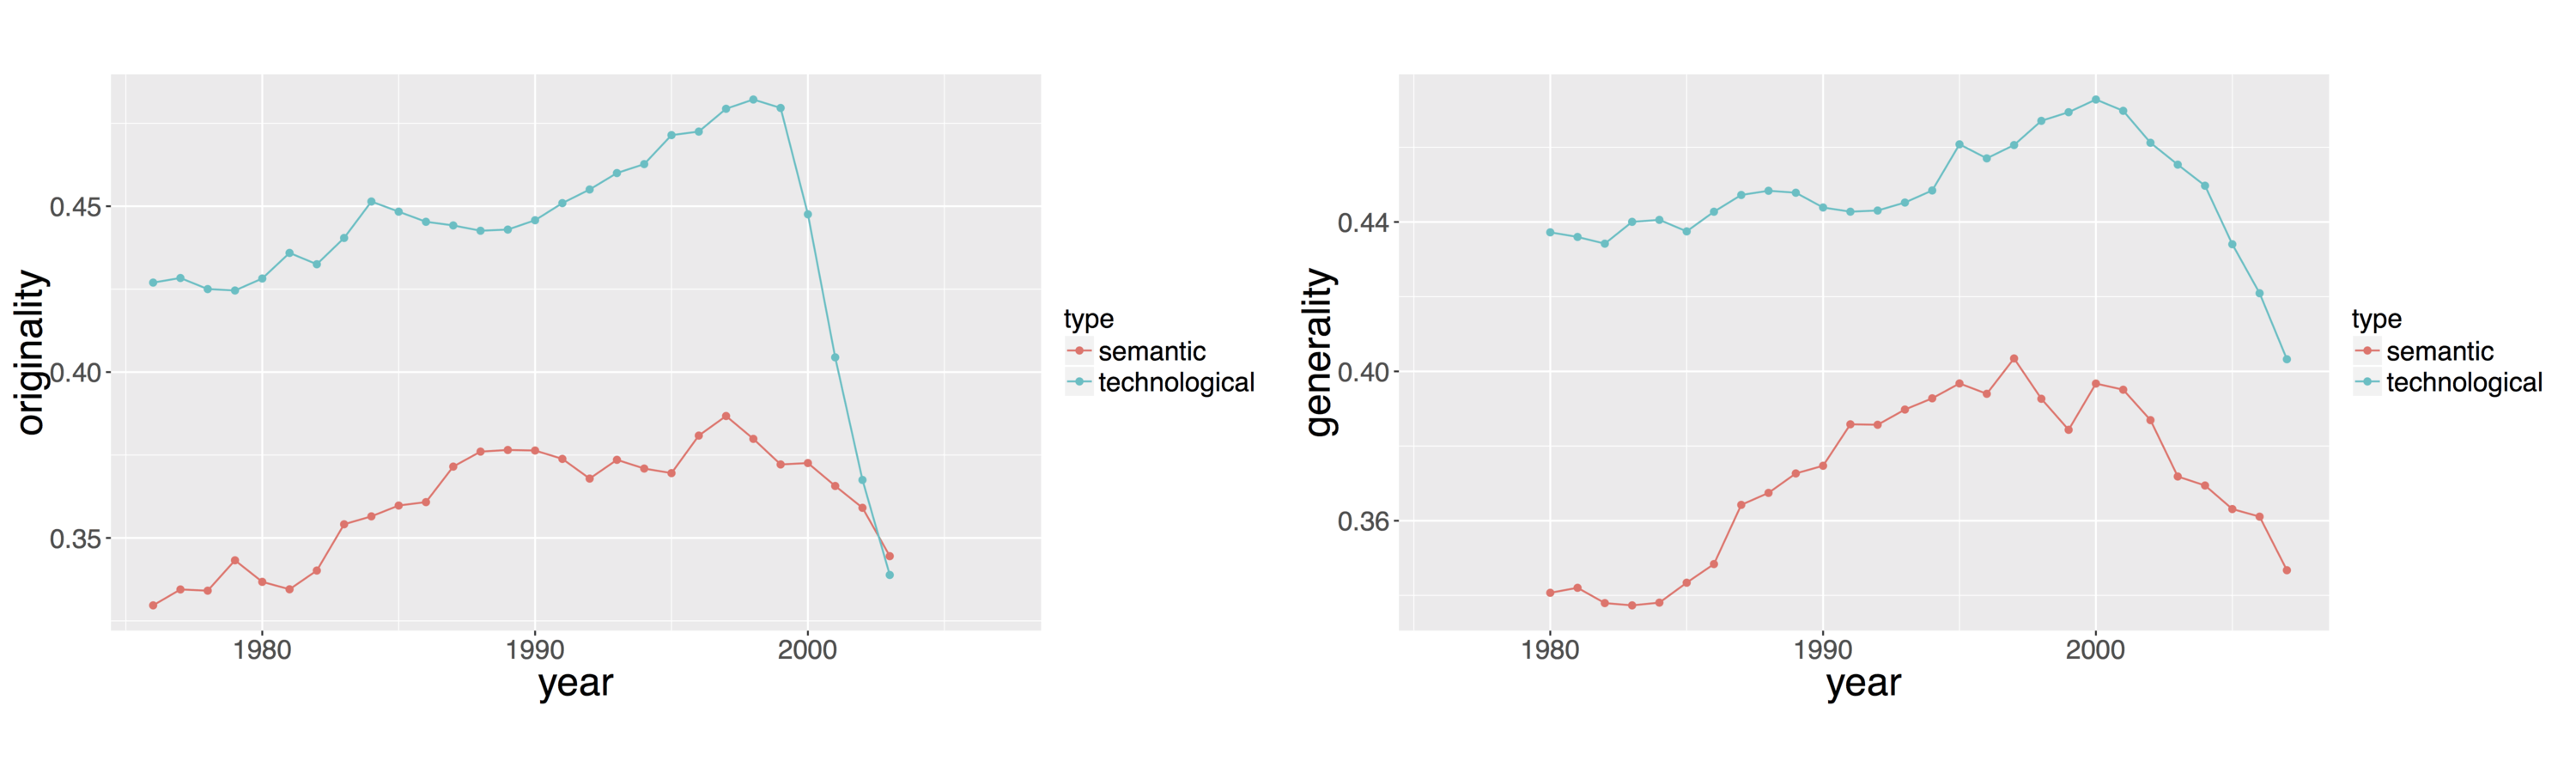
\includegraphics[width=\textwidth]{figures/Fig6.png}
    
    \medskip
    
    \textit{Systematically lower originality and generality (citation-based measures) for the semantic classification (consistent with the higher modularity shown thereafter).}
    
\end{frame}

\begin{frame}{Stochastic Block Modeling to evaluate consistency of classifications}
\begin{itemize}
    \item   We complete the analysis by developing a statistical model aiming at quantifying performance of both technological and semantic classification systems
    \item Intuitively, we look at within class citations proportion (for both technological and semantic approaches)
    \item Question: is the semantic classification better at predicting future within class citations? \\
    $\longrightarrow$ short answer is \alert{yes}.
\end{itemize} 
\end{frame}




\begin{frame}{Network sensitivity analysis}
\label{slide:sensitivity}
\hyperlink{slide:relevance}{\beamerbutton{Back}}

	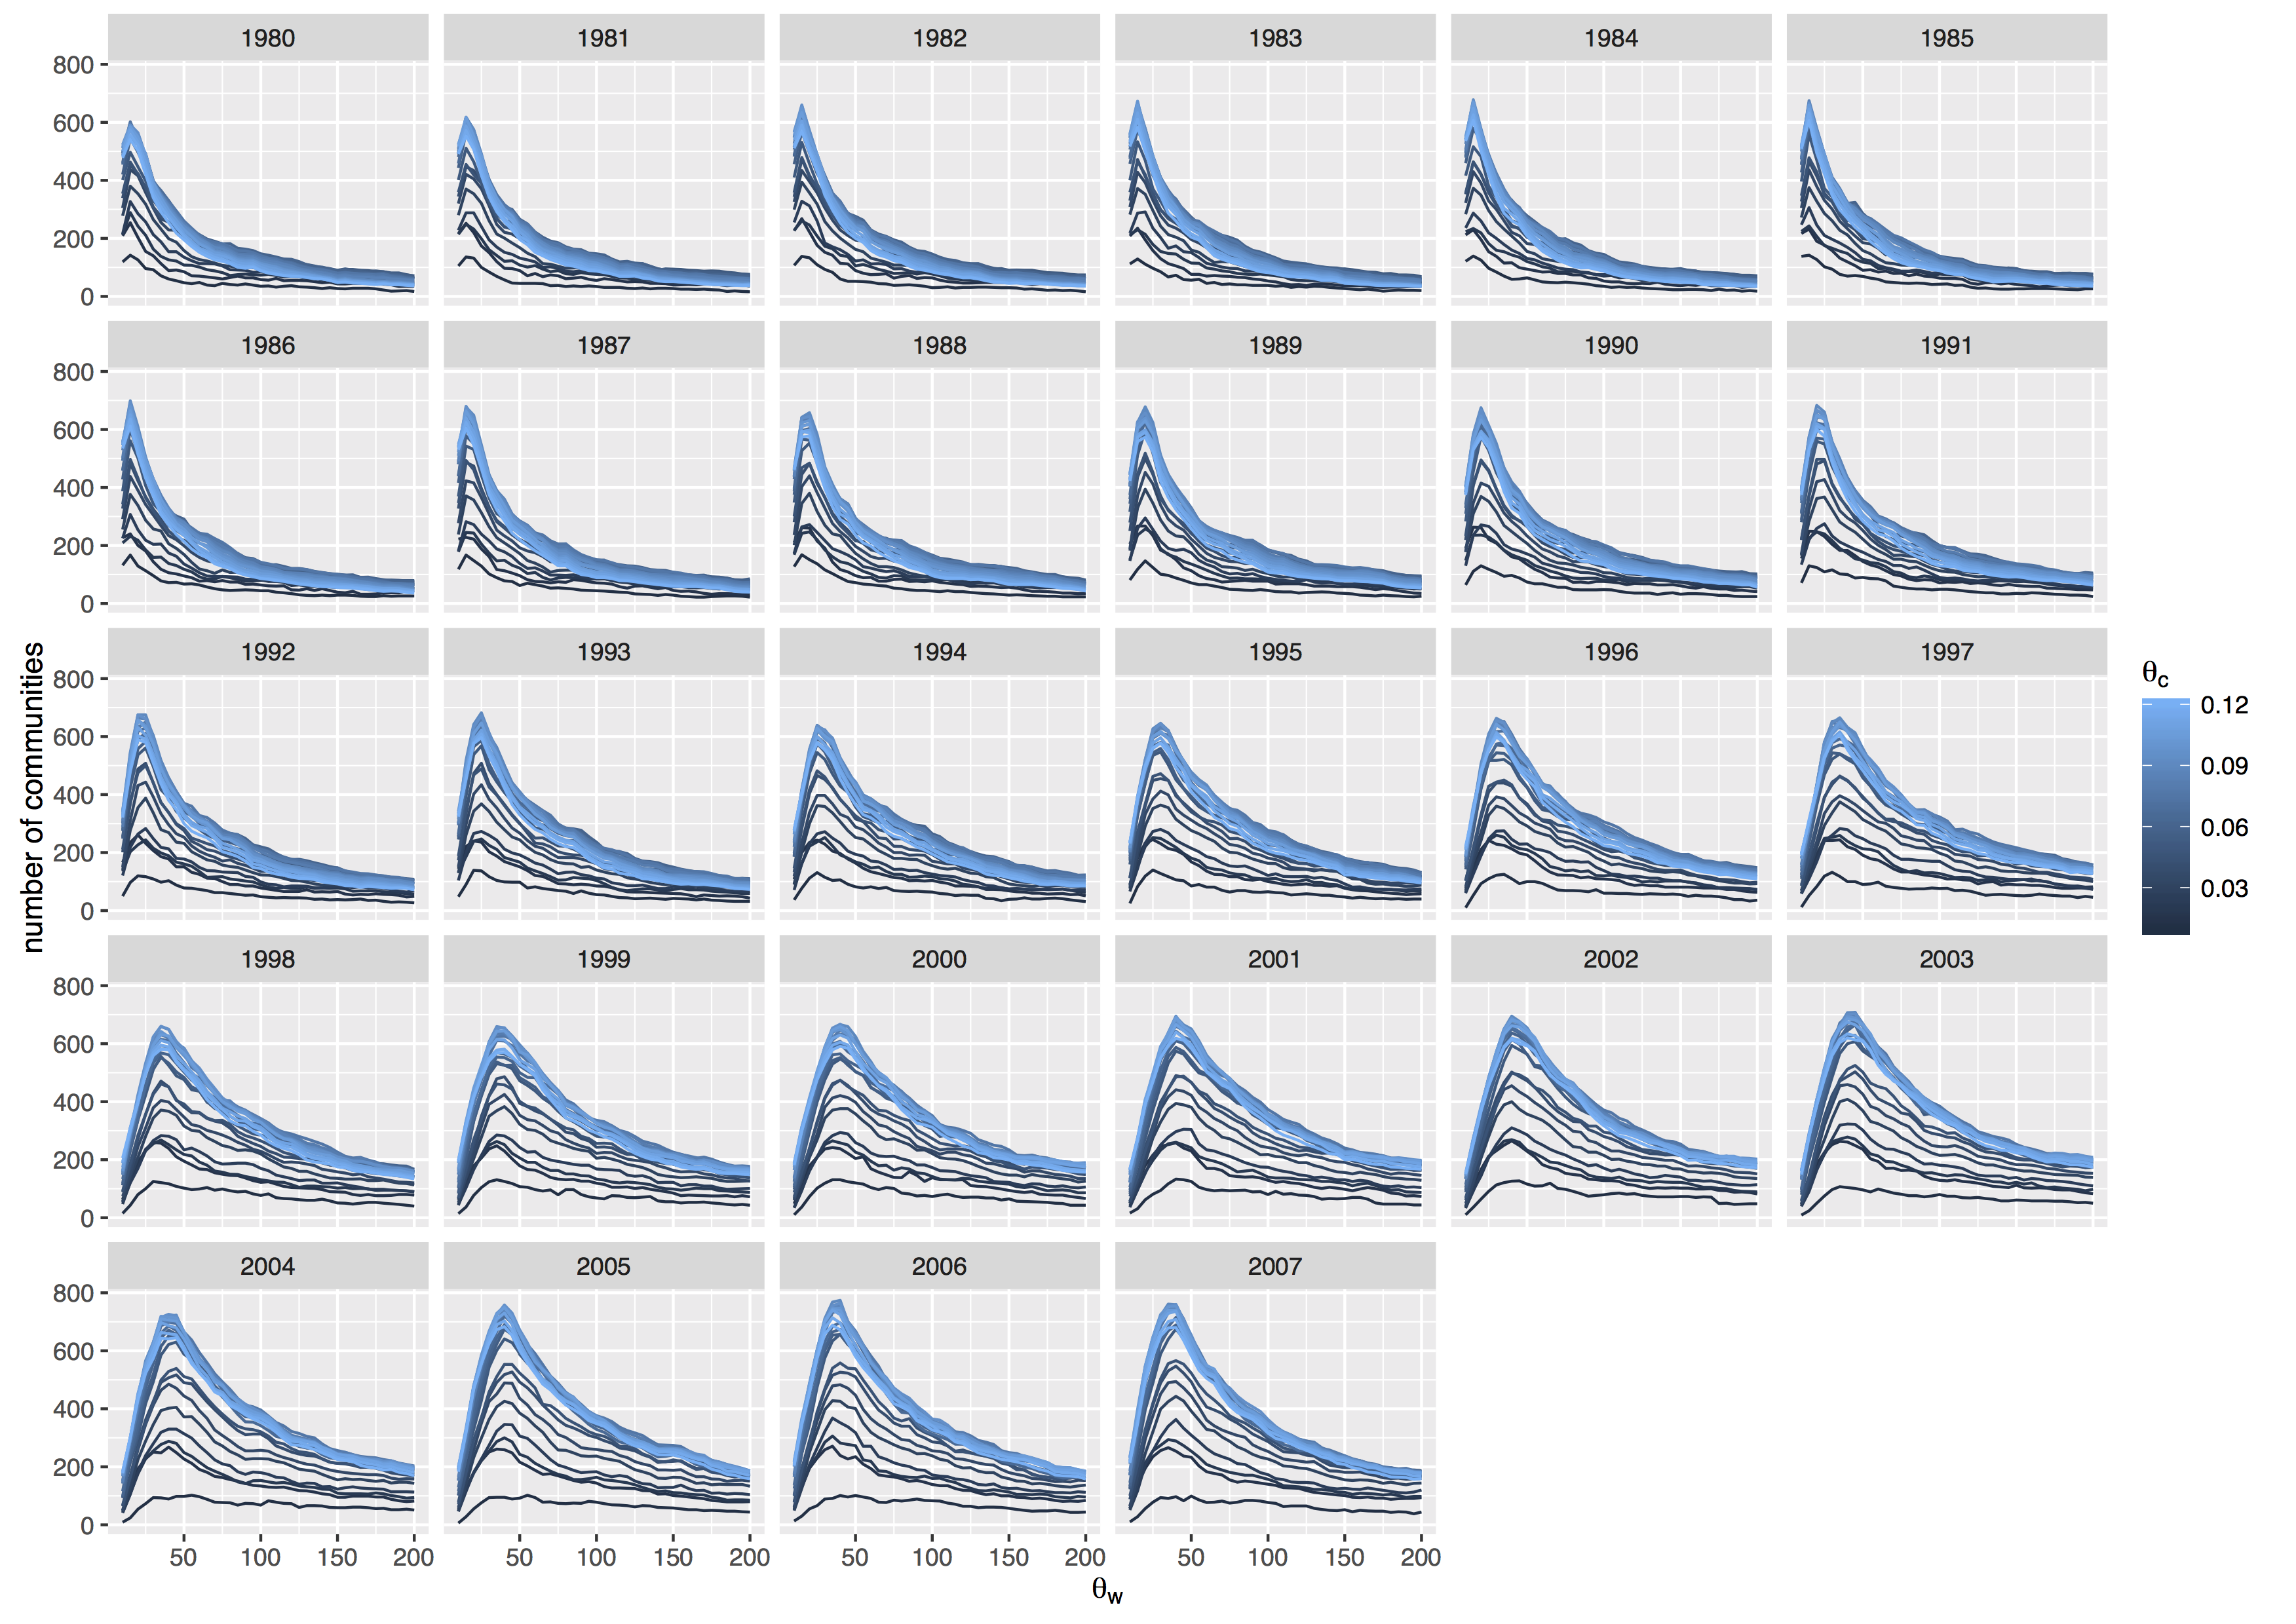
\includegraphics[width=\textwidth]{figures/commnum_thetaw_byyears.png}
\end{frame}


\begin{frame}{Network sensitivity analysis ($T_W = 2$)}
	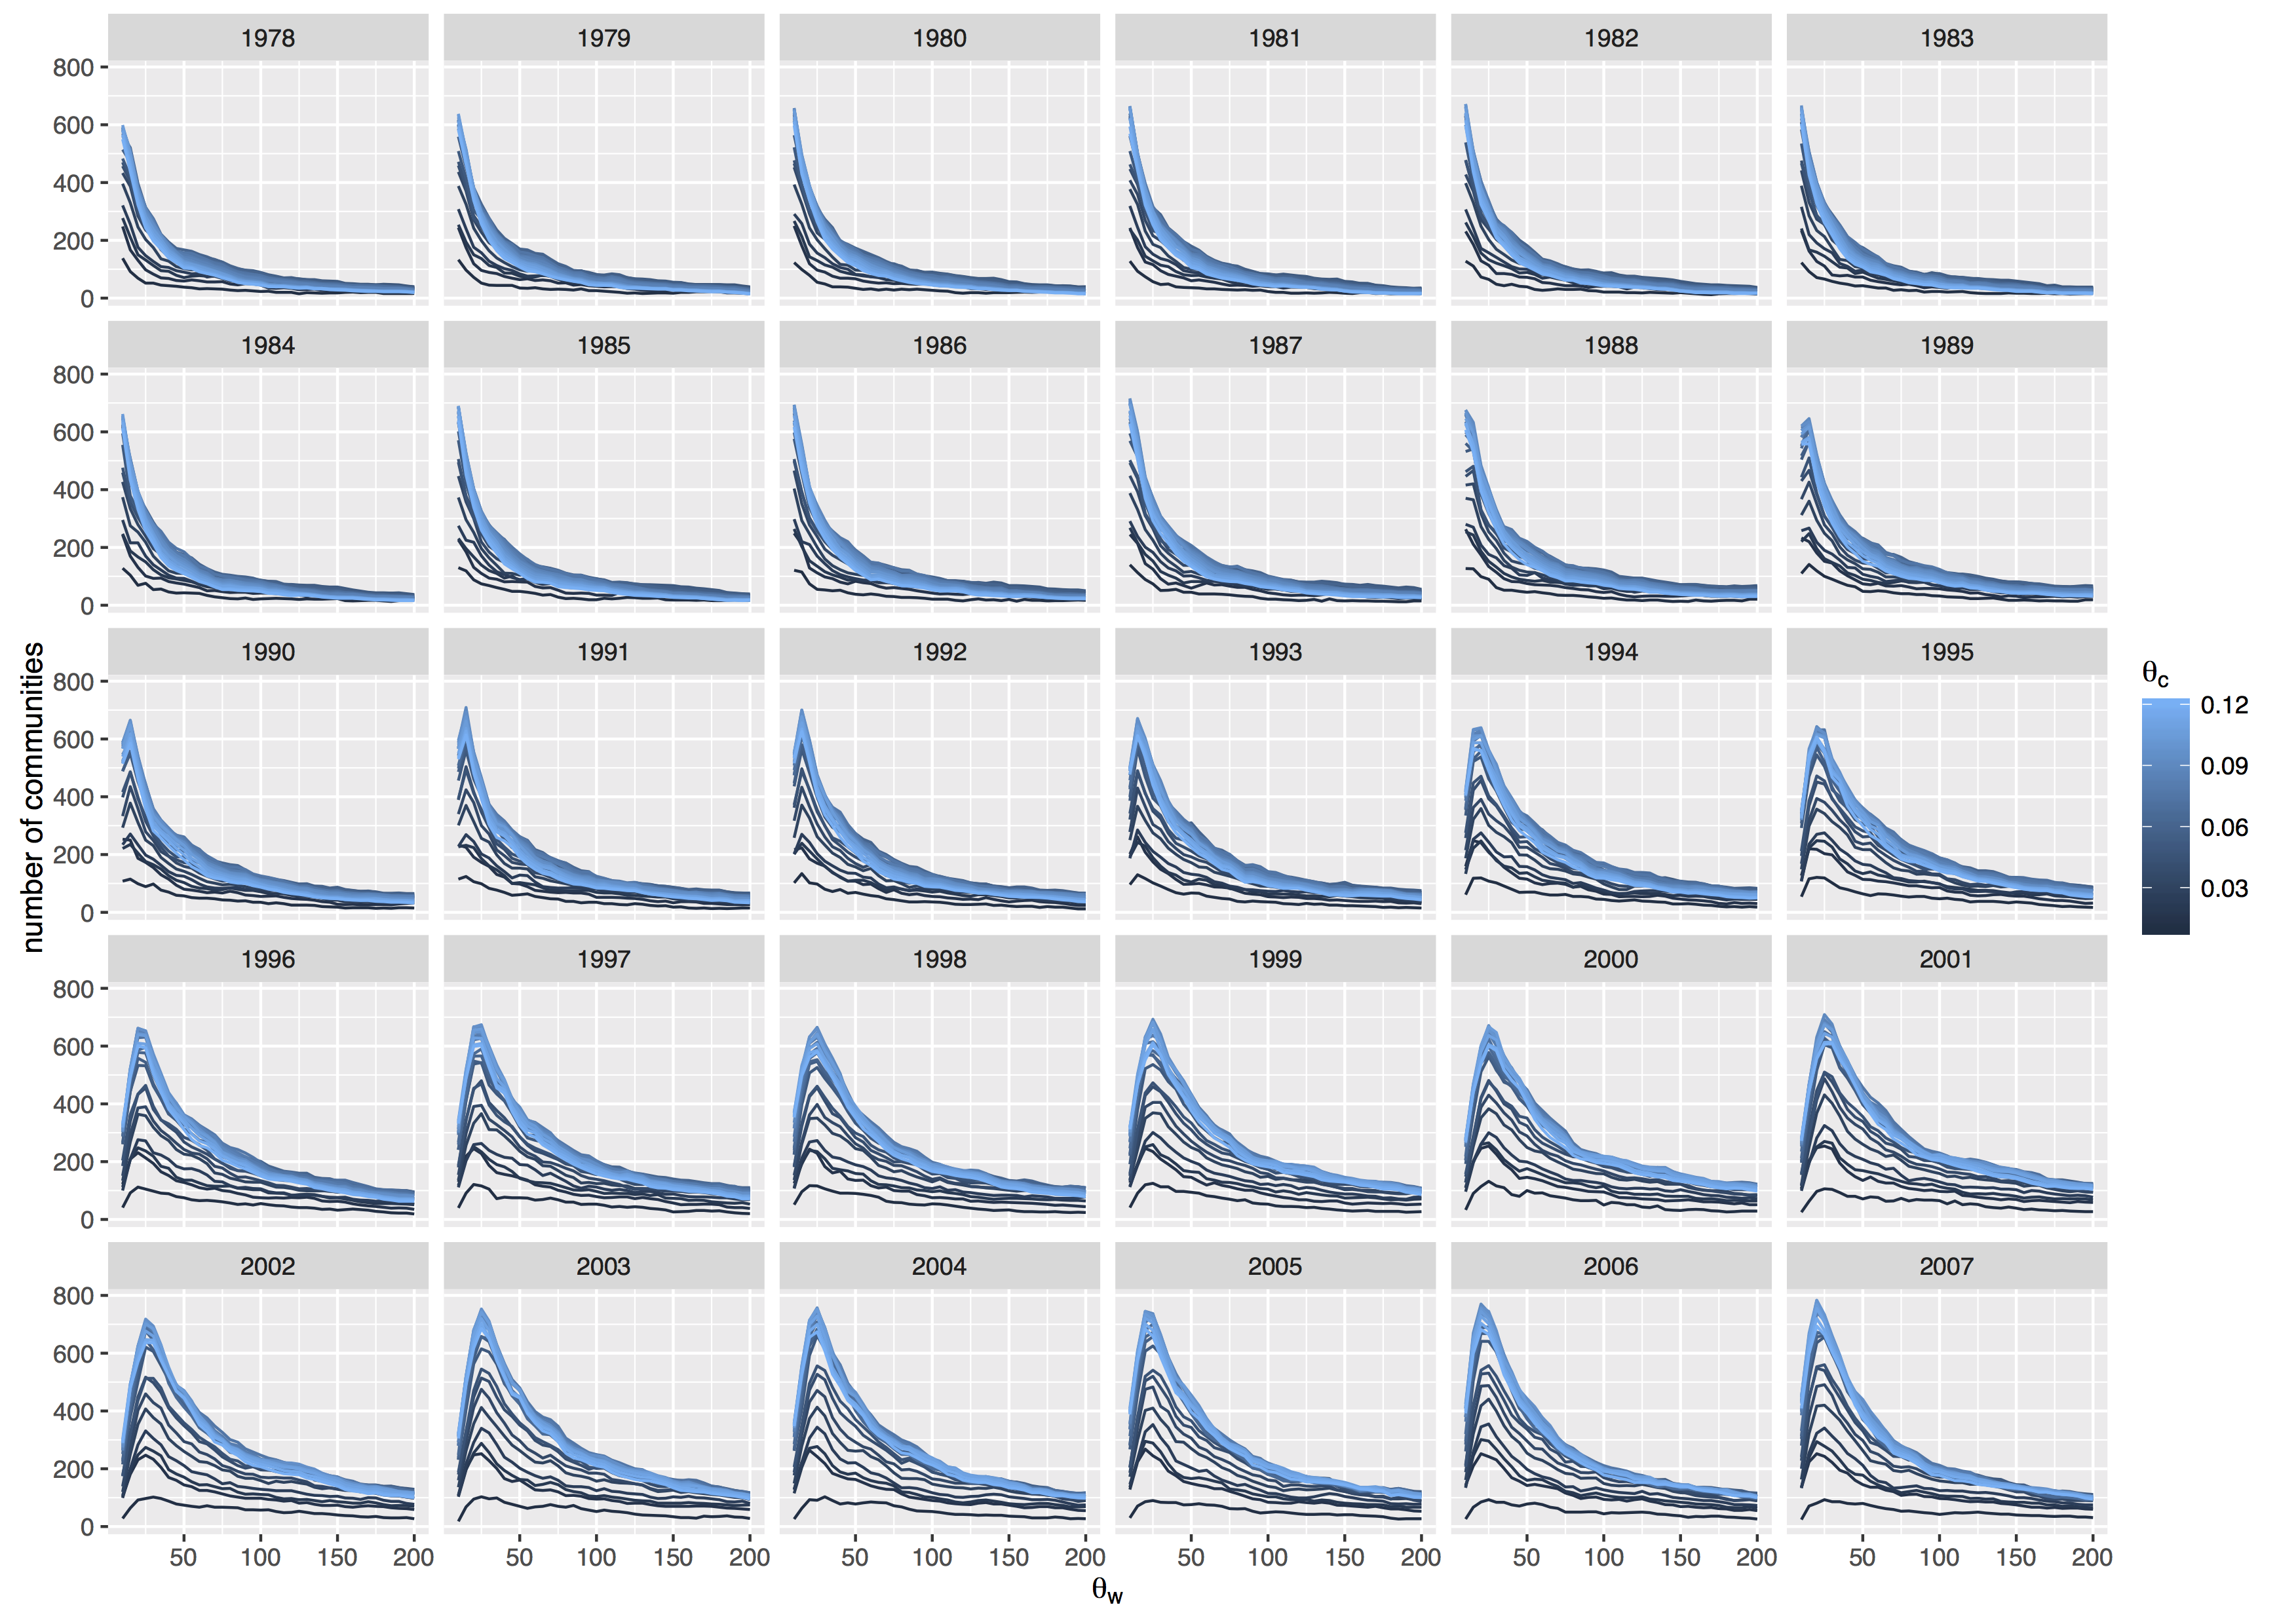
\includegraphics[width=\textwidth]{figures/commnum_thetaw_byyears_window3.png}
\end{frame}


\begin{frame}{Network sensitivity analysis}
	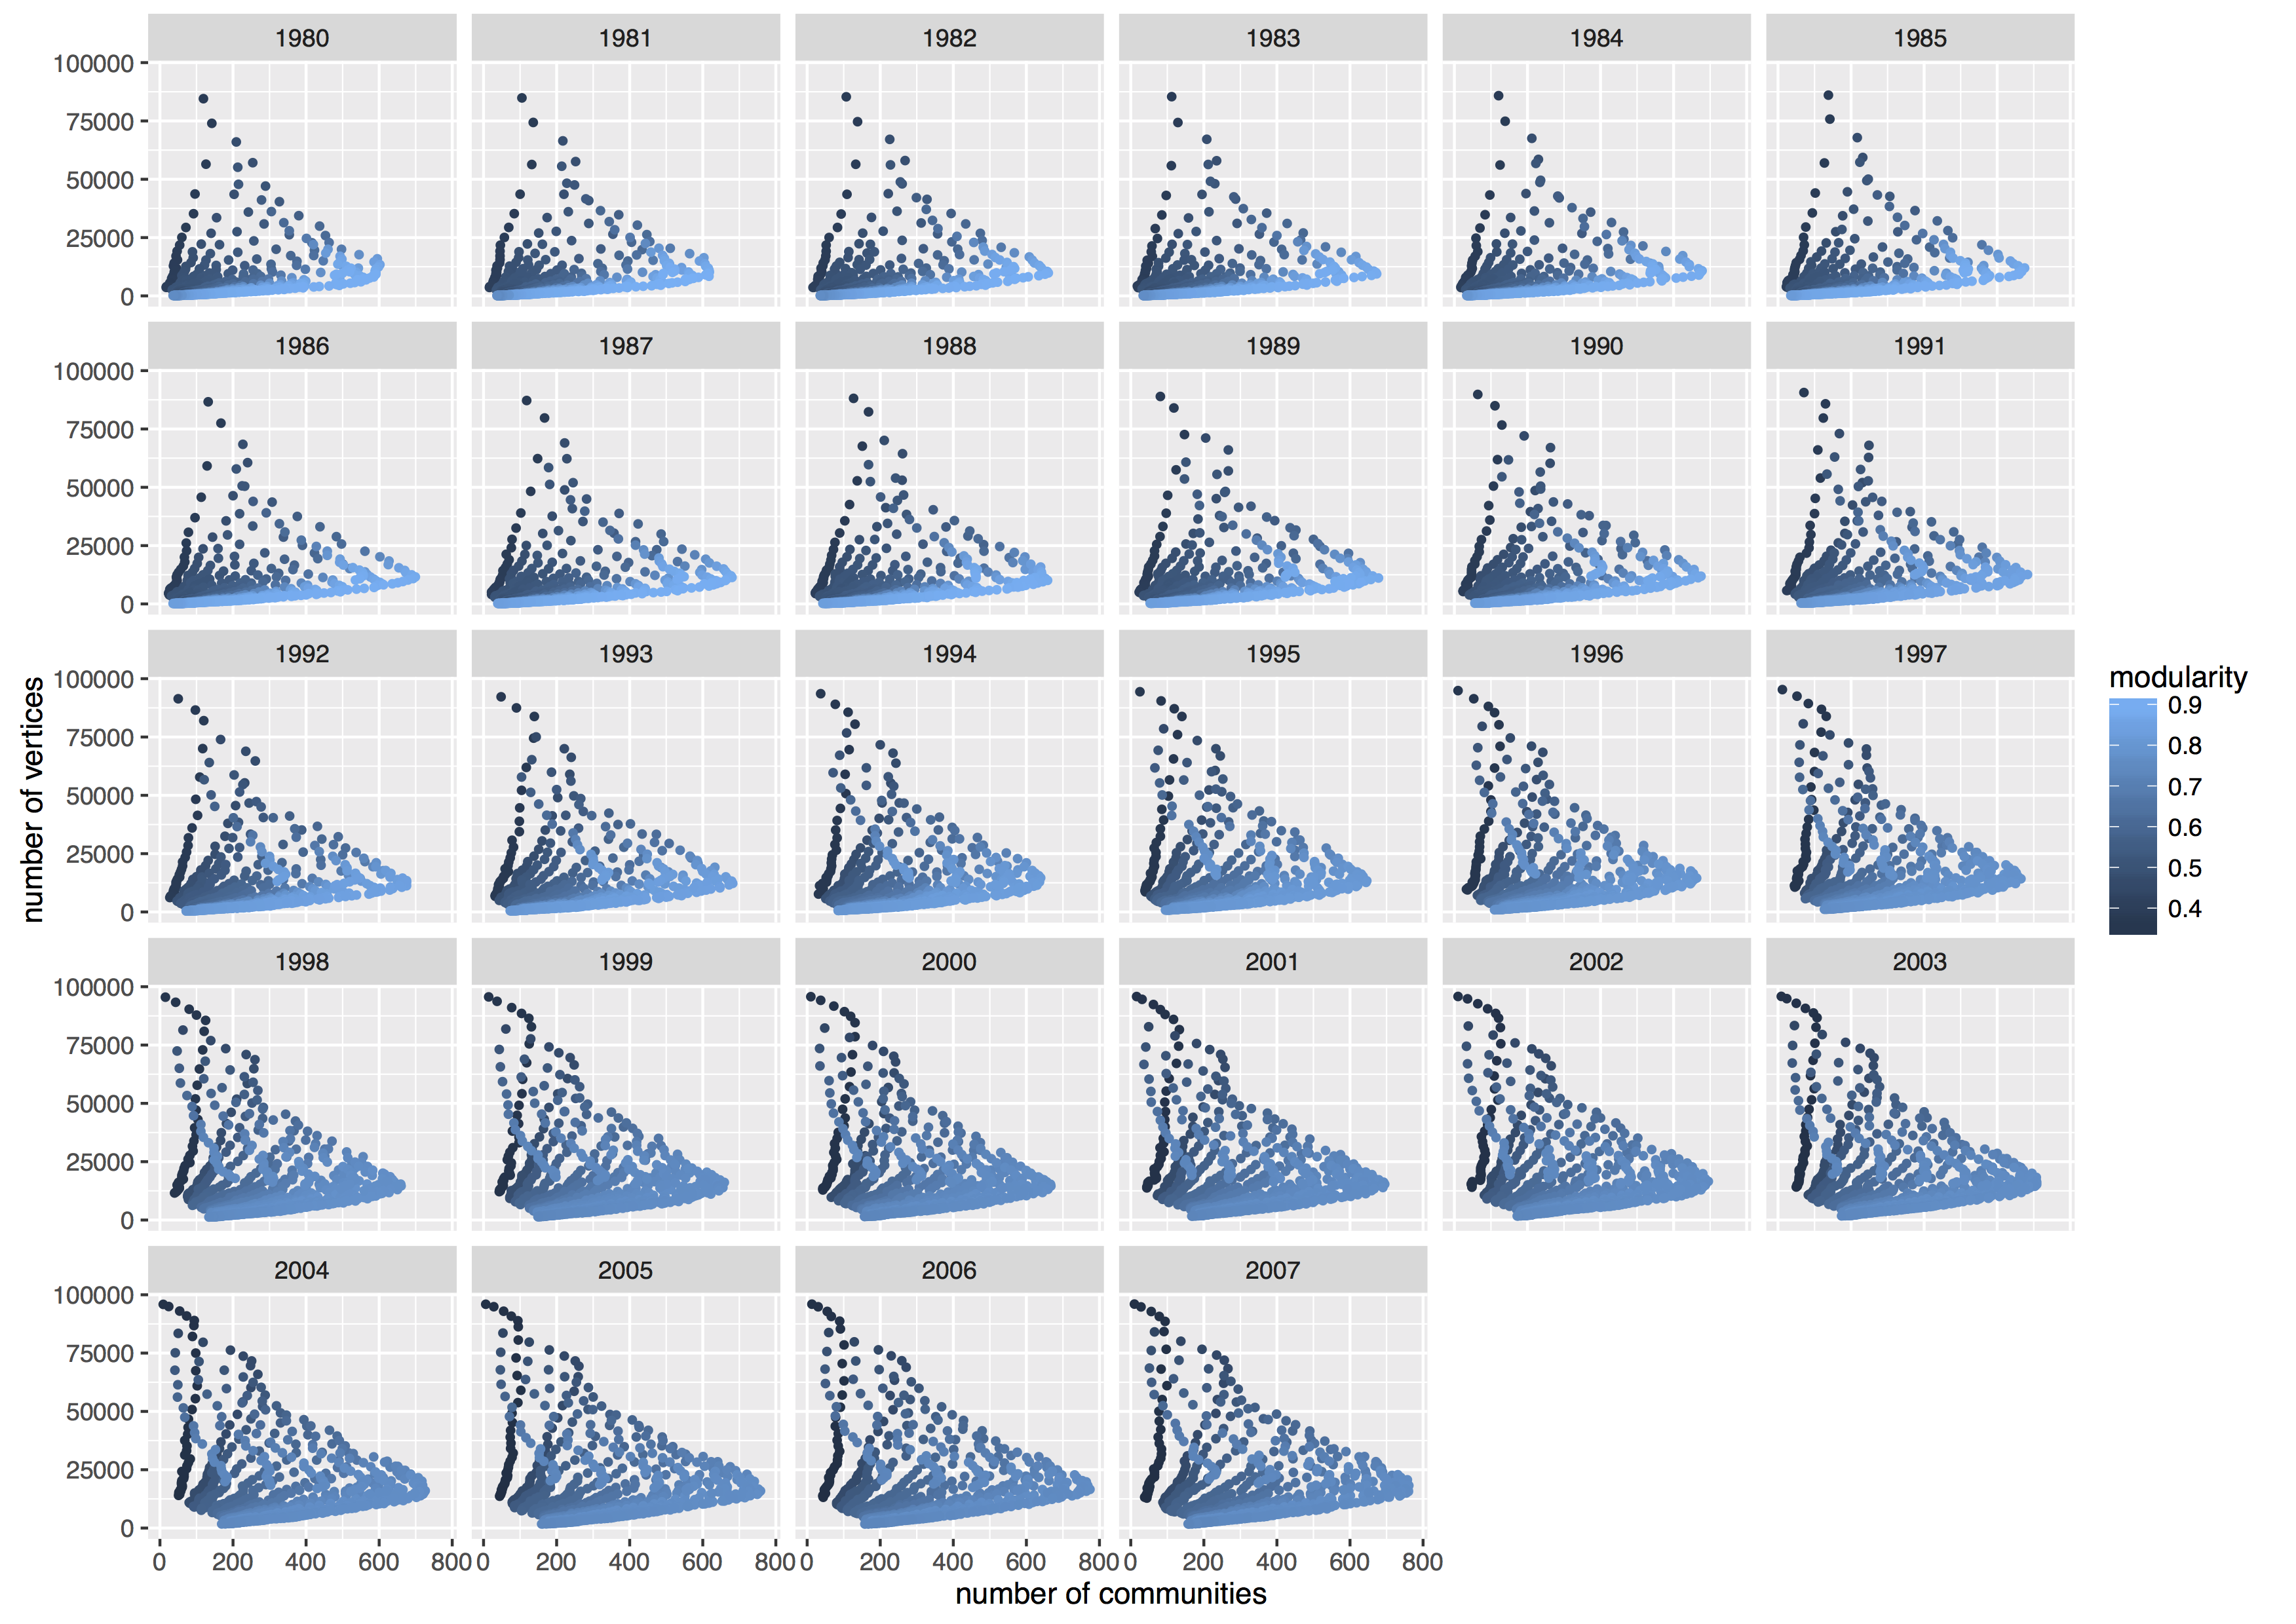
\includegraphics[width=\textwidth]{figures/vcount_comnum_pareto.png}
\end{frame}


\begin{frame}{Network sensitivity analysis ($T_W = 2$)}
	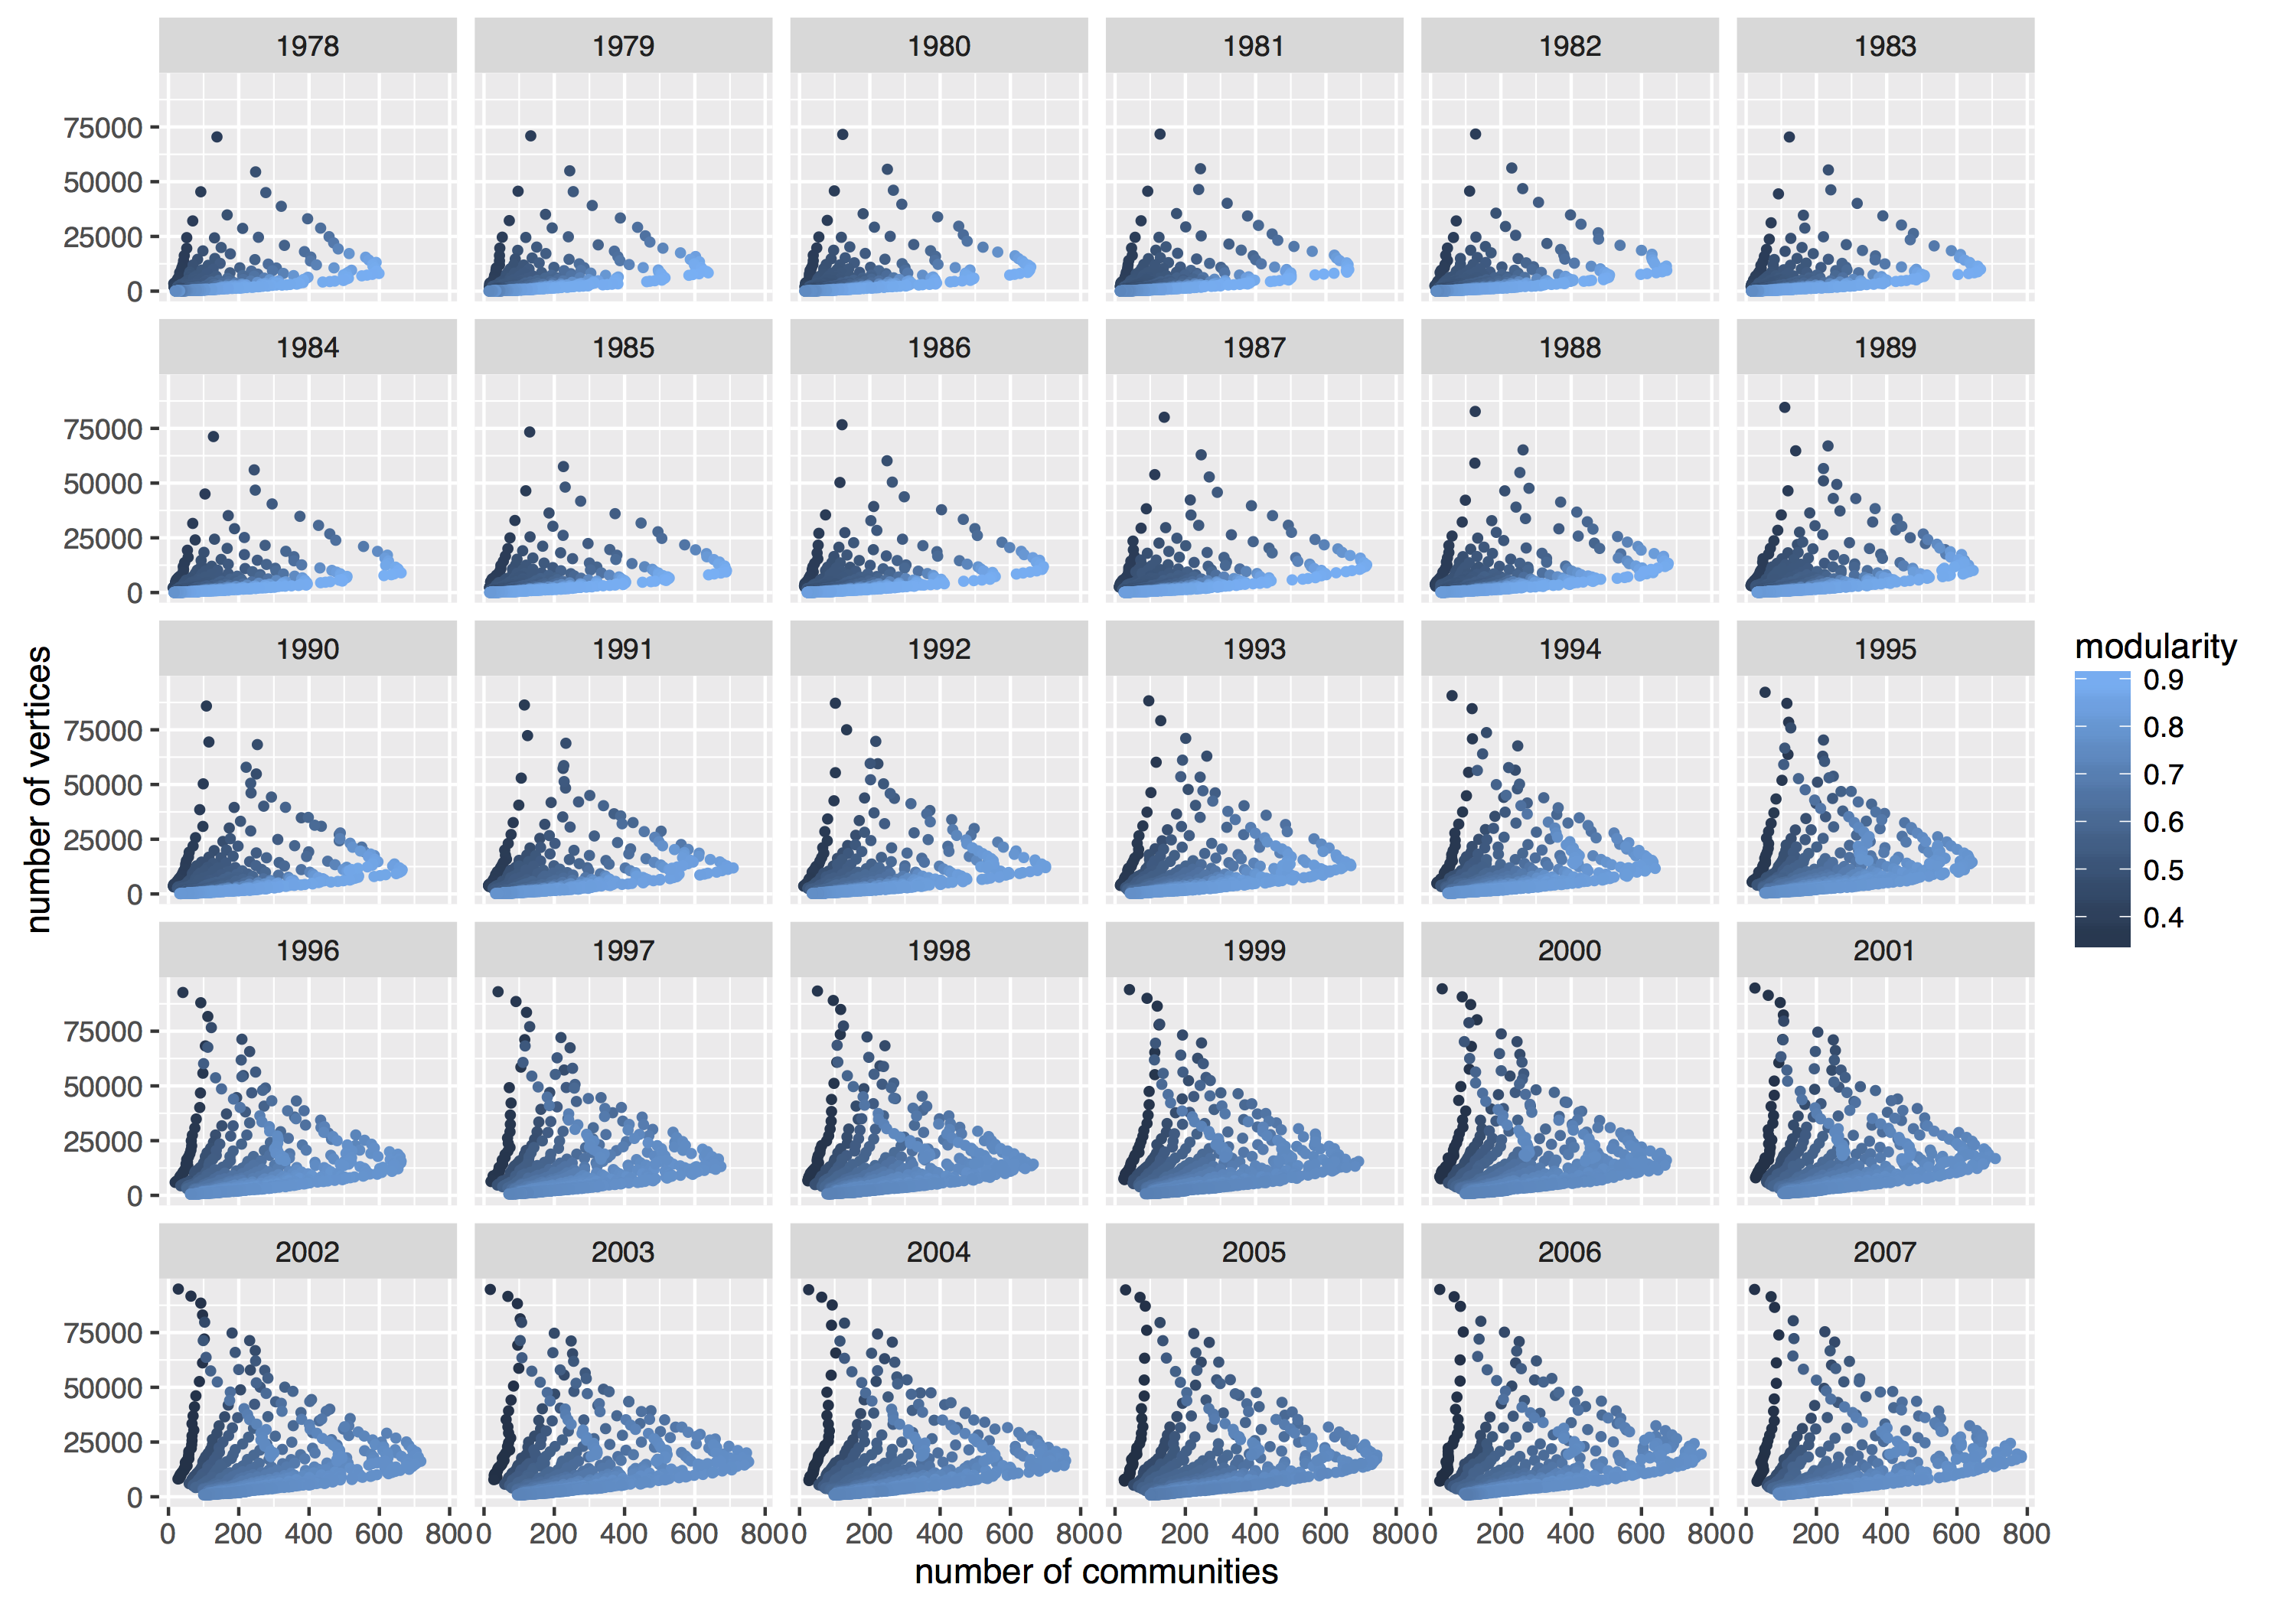
\includegraphics[width=\textwidth]{figures/vcount_comnum_pareto_window3.png}
\end{frame}


\begin{frame}{Network sensitivity analysis}
	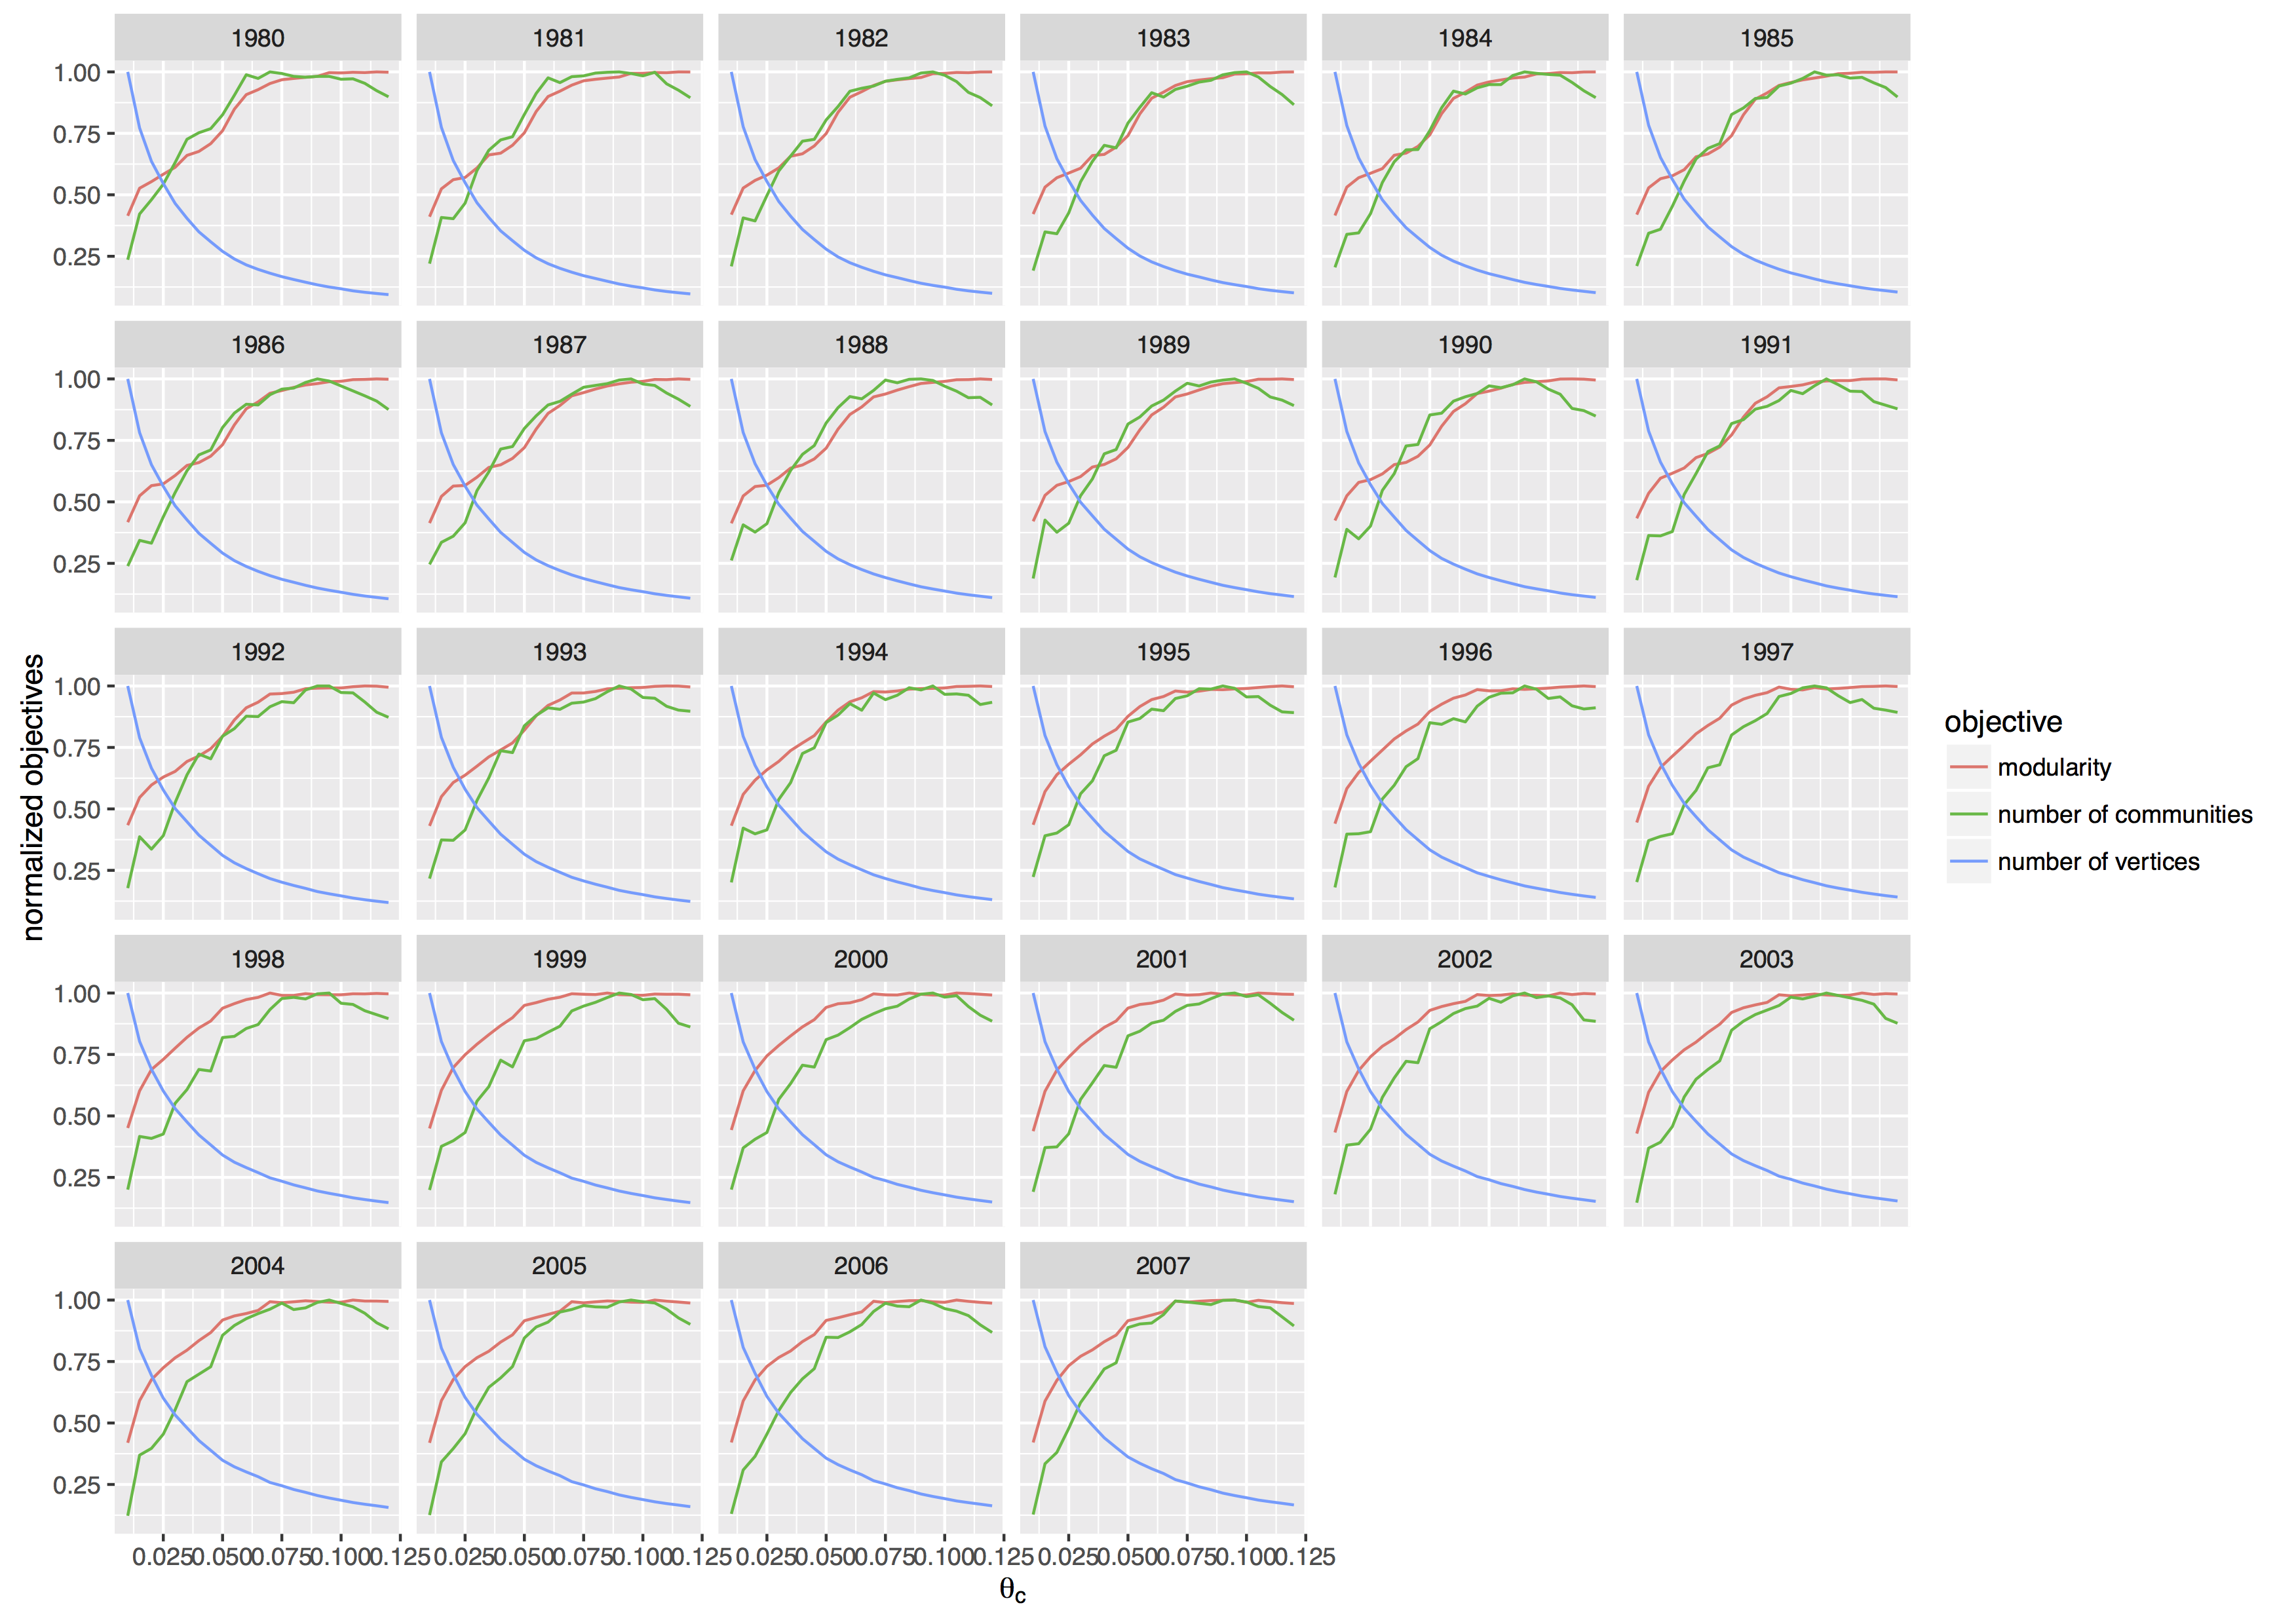
\includegraphics[width=\textwidth]{figures/normalizedObjs-dispth_eth4_1e-5.png}
\end{frame}


\begin{frame}{Network sensitivity analysis ($T_W = 2$)}
	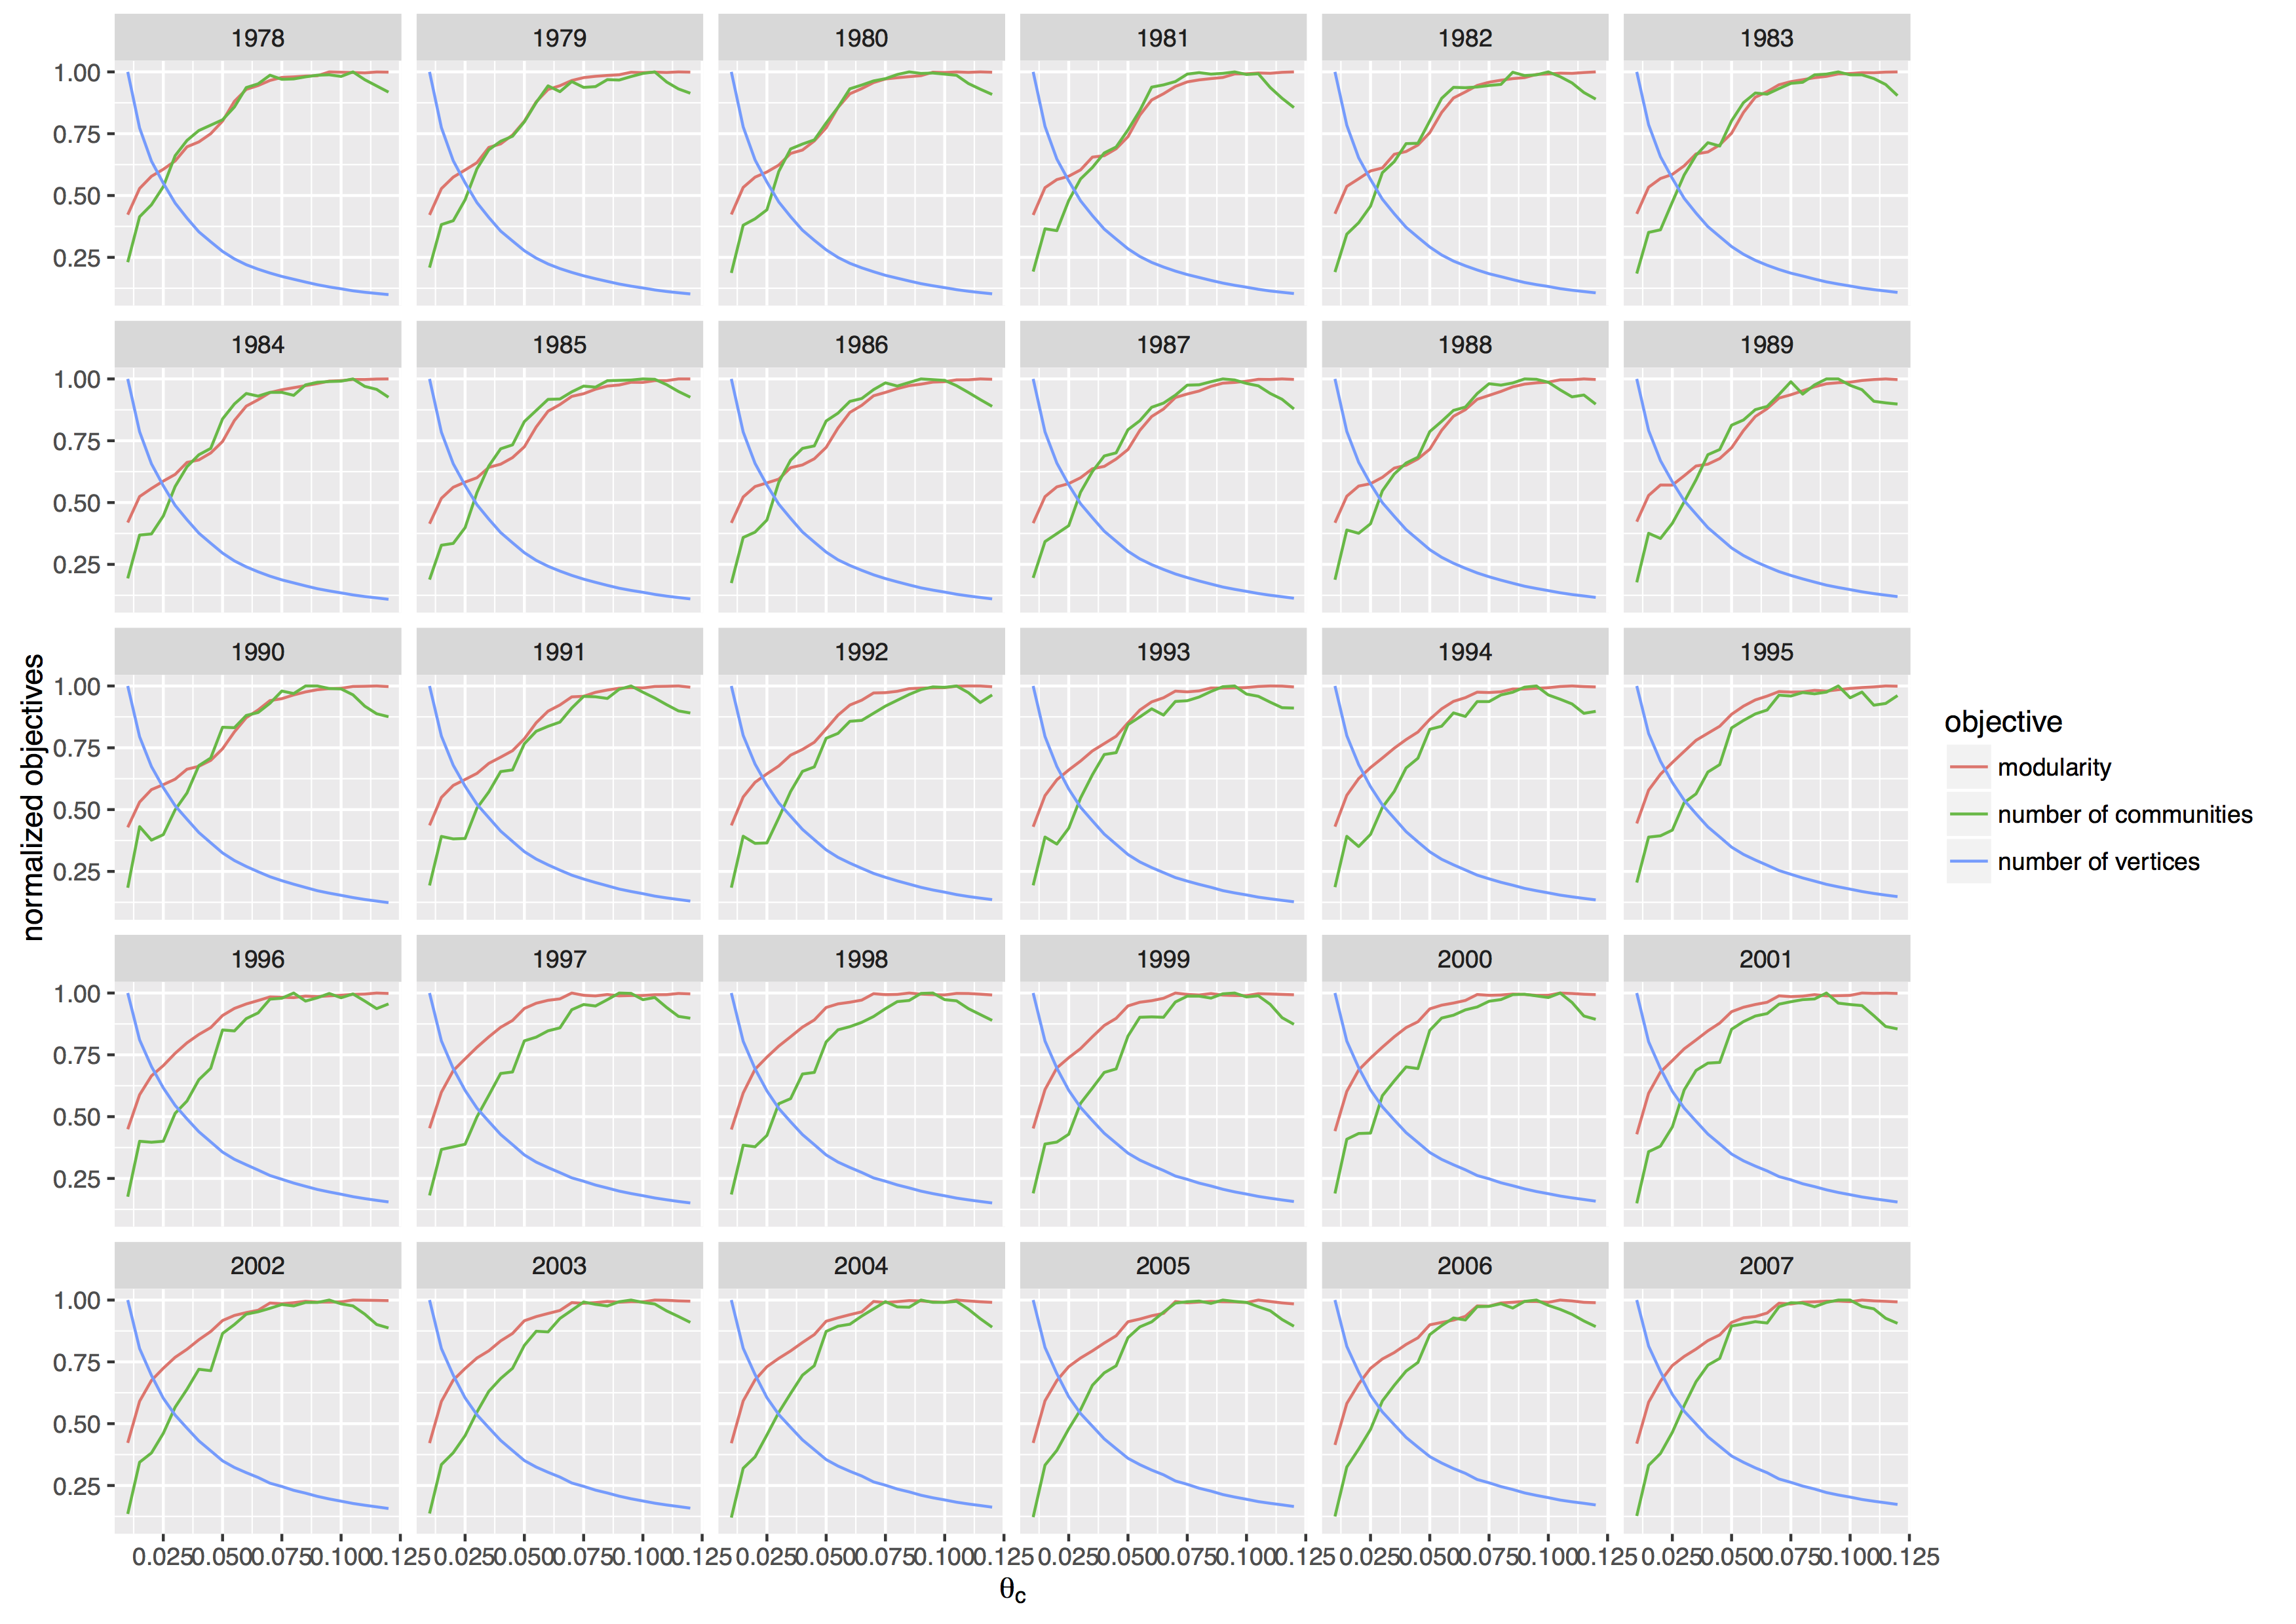
\includegraphics[width=\textwidth]{figures/normalizedObjs-dispth_window3_eth4_1e-5.png}
\end{frame}










%%%%%%%%%%%%%%%%%%%%%
\begin{frame}[allowframebreaks]
\frametitle{References}
\bibliographystyle{apalike}
\bibliography{patents}
\end{frame}
%%%%%%%%%%%%%%%%%%%%%%%%%%%%



\end{document}